\documentclass[a4paper, 11pt]{article}
\usepackage{jheppub}
\usepackage[compat=1.1.0]{tikz-feynman}
\usepackage{float}
\usepackage{bm}
% Disable LuaTeX warning about automatic vertex placement
\tikzfeynmanset{warn luatex=false}
\usepackage{amsmath, amssymb}   % you probably already have these
\usepackage{slashed}            % for Feynman slash notation \slashed{p}

\title{\boldmath Symmetry Protection and the Hierarchy Problem: From Lattice Models to Goofy}
\author{Juana Granados Rodríguez,}
\affiliation{Facultat de F\'{\i}sica, Universitat de Barcelona, Martí i Franquès 1, 08028 Barcelona, Spain.}
\emailAdd{jgranaro19@alumnes.ub.edu}
\author{Advisor: Dr. Jordi Salvadó Serra}

\abstract{The hierarchy problem asks why the Higgs mass remains so far below the high-energy scales at which new physics is expected, despite quantum corrections that tend to drive it upward. It can be reformulated as a question of symmetry because a parameter is stable under radiative corrections when setting it to zero enlarges the symmetry of the theory. We examine this principle of symmetry protection in two complementary settings. First, in a two-dimensional Ising model, extending an existing inverse-Ising blocking procedure to $\mathbb{Z}_2$-odd operators, we show numerically that such operators are generated under coarse-graining only when the symmetry is explicitly broken. We then revisit one-loop mass corrections in quantum field theory, contrasting the fermion self-energy, whose mass correction vanishes in the chiral limit, with the scalar self-energy, which has no analogous protection. This identifies the hierarchy problem as the absence of a symmetry forbidding a generic scalar mass operator. Finally, we review the \textit{goofy} symmetry, a transformation acting non-trivially on kinetic terms that can forbid the Higgs mass while remaining compatible with the Standard Model.
\\

\noindent\textsc{Resum:} El problema de la jerarquia es pregunta per què la massa de Higgs roman fins ara tan per sota de les escales d'alta energia on s'espera nova física, malgrat les correccions quàntiques que tendeixen a elevar-la. Es pot reformular com una qüestió de simetria perquè un paràmetre és estable sota les correccions radiatives quan establir-lo a zero amplia la simetria de la teoria. Examinem aquest principi de protecció de la simetria en dos entorns complementaris. En primer lloc, en un model d'Ising bidimensional, en estendre un procediment de bloqueig d'Ising invers existent a operadors imparells respecte a $\mathbb{Z}_2$, mostrem numèricament que aquests operadors es generen sota el granulat només quan la simetria es trenca explícitament. A continuació, revisitem les correccions de massa d'un bucle a la teoria quàntica de camps, contrastant l'autoesenergia dels fermions, la correcció de massa de la qual desapareix en el límit quiral, amb l'autoesenergia escalar, que no té una protecció anàloga. Això identifica el problema de la jerarquia com l'absència d'una simetria que prohibeixi un operador de massa escalar genèric. Finalment, revisem la simetria \textit{goofy}, una transformació que actua de manera no trivial sobre els termes cinètics i que pot prohibir la massa de l'Higgs, tot i mantenir-se compatible amb el Model Estàndard.}

\keywords{Theoretical physics, Quantum field theory, High energy physics, Elementary particles, Statistical mechanics, Quantum theory}


\begin{document}
\maketitle
\section{Introduction}
\label{sec:intro}

The hierarchy problem is considered one of the main hints of physics beyond the Standard Model. Essentially, it asks why the Higgs boson is so much lighter than the Planck scale when quantum corrections to its mass would naively be expected to make it comparable to the scale at which new physics appears, unless we perform a fine tuning to cancel these contributions \cite{PeskinHierarchy}. In this work we explore how the discovery of a new symmetry could provide another candidate solution to this problem. This candidate is the recently proposed ``goofy'' symmetry \cite{2HDM, Trautner_goofy1, goofy2}, which offers a natural explanation for why the Higgs mass remains small without requiring fine-tuning.

To motivate the introduction of the \textit{goofy} symmetry, it is useful to review the role of symmetries in protecting small parameters in quantum field theory. A well-known example is provided by fermion masses, which are protected by chiral symmetry. Setting the fermion mass to zero enlarges the symmetry of the theory and this is what makes a small mass \emph{natural} in the sense of 't Hooft \cite{CraigNaturalness}. By contrast, setting scalar mass terms to zero does not, in general, restore an internal or gauge symmetry \cite{wilson}. Scalar masses are therefore not protected by symmetry in the same way as fermion masses and are sensitive to ultraviolet physics. This absence of symmetry protection for the Higgs mass underlies the hierarchy problem and motivates the search for alternative symmetries that could protect the Higgs mass in analogy with chiral symmetry. Recent work suggests that \textit{goofy} transformations may provide such a mechanism.

This symmetry, initially called the $r_0$-symmetry, was first identified by Ferreira, Grzadkowski, Ogreid and Osland \cite{2HDM}, who found a relation between couplings in the two-Higgs-doublet model (2HDM) that is both basis-independent and preserved by the renormalization group (RG) to all orders in perturbation theory, but it had not been considered due to its unusual characteristics and the problems it raised. The transformation was later renamed the \emph{GOOFy} transformation by Ferreira \cite{FerreiraHPNP2023}, a name that reflects both its unusual nature and the initials of the original authors arranged in a playful ``rotation'' hinting the action of the transformation on the components of the Higgs doublet. Trautner \cite{Trautner_goofy1} and Boer, Goertz and Incrocci \cite{goofy2}, later reinterpreted this relation as the invariance of the theory under a transformation of the fields, $H \to iH$ and extended the idea to the Standard Model. The transformation is admittedly peculiar, for it is imaginary and it is not obvious how to embed it in a conventional spacetime symmetry structure. What makes it interesting is the fact that the relation between couplings survives the RG flow to all orders, supporting the claim that it is a symmetry, even if its geometric interpretation is not yet clear \cite{2HDM, Trautner_goofy1, goofy2, deBoer_Trautner_Outs}. 


Motivated by these ideas, the goal is to understand in a more intuitive level the hierarchy problem by exploring the general principle of symmetry protection, which is the underlying mechanism that makes the \textit{goofy} interesting in the first place. For this, we will use some simulations to study a lattice toy Ising model by adding symmetry-breaking operators into the numerical calculation of the RG flow (as it was done by Di Carlo \cite{blocking} only for symmetry-preserving operators) to see the same protection mechanism at work in a non-perturbative yet more intuitive setting. Furthermore, to properly connect it to the \textit{goofy} transformation, we will revisit the standard QFT calculations of mass corrections for fermions and scalars, with the explicit aim of seeing how the symmetry shows up in the result. 

The hope is that, by the end, the slogan ``symmetry protects mass'' will feel less like a slogan and more like something one can see happening, both in Feynman diagrams and in lattice flows. Seen in this light, \textit{goofy} is not only an exotic curiosity but a natural candidate to play, for the Higgs, the role that chiral symmetry plays for fermions.


\subsection{Renormalization Group Basic Concepts}
\label{sec:RG_intro}

The renormalization group (RG) provides a framework for understanding how the effective description of a physical system changes with scale \cite{Goldenfeld, Cardy}. In general, short-distance degrees of freedom are progressively integrated out, producing a sequence of effective theories that describe the same physics at increasingly larger length scales \cite{TongSFT}.

It is useful to think of all possible theories as points in an abstract theory space. Each axis corresponds to the coupling associated with an operator allowed by the symmetries of the system. An RG transformation moves the theory from one point in this space to another, generating an \textit{RG flow}.

Particularly important are the points that remain invariant under the transformation. These are called \textit{fixed points}. Near a fixed point, one can linearize the RG transformation and classify operators according to how their couplings behave under a change of scale,
\begin{equation*}
g_i' = b^{y_i} g_i ,
\end{equation*}
where $b>1$ is the rescaling factor and $y_i$ is the scaling exponent associated with the coupling $g_i$ \cite{Goldenfeld,Cardy}. Operators are then classified as:
\begin{itemize}
\item \textbf{Relevant} ($y_i>0$): their couplings grow toward the infrared and drive the theory away from the fixed point.
\item \textbf{Irrelevant} ($y_i<0$): their couplings become progressively less important at long distances.
\item \textbf{Marginal} ($y_i=0$): their couplings remain unchanged at leading order and require a more detailed analysis.
\end{itemize}

Since most microscopic operators are irrelevant, the long-distance behavior of a system depends only on a small number of relevant directions \cite{TongSFT}. Consequently, physically distinct systems can flow toward the same fixed point and exhibit identical large-scale behavior despite possessing very different microscopic descriptions \cite{Goldenfeld, Cardy}.

For the purposes of this work, an additional property of the RG is particularly important. Renormalization preserves the symmetries of the theory. If a symmetry forbids a given operator, then the RG flow cannot generate that operator as long as the symmetry remains exact. Geometrically, the flow is confined to a symmetry-preserving subspace of theory space. Conversely, once the symmetry is explicitly broken, the RG is free to explore previously forbidden directions.

This observation provides the common language that connects the remainder of this thesis. In the Ising model, the $\mathbb{Z}_2$ symmetry protects odd-spin operators from being generated under coarse-graining. In quantum field theory, chiral symmetry protects the fermion mass operator from large radiative corrections. Finally, the motivation behind \textit{goofy} transformations is the possibility that a new symmetry principle may similarly protect the Higgs mass operator. In all three cases, the central question is ultimately the same: how do symmetries constrain the allowed directions of the RG flow?


\section{Symmetry Protection in the Ising Model} % ~5 pages
\label{sec:ising}

For a more tangible picture of the symmetry protection mechanism, we begin by looking at the 2D Ising model. This model has a $\mathbb{Z}_2$ symmetry that protects certain operators from being generated under RG flow and provides a nice playground to see how this works in practice. We will first motivate the Ising Model setup, introduce the necessary theoretical background and then follow an extended version of the blocking method of Di Carlo \cite{blocking} to compute the RG flow of the couplings and two newly introduced odd operators (that break the $\mathbb{Z}_2$ symmetry) in the Hamiltonian. This with the aim of seeing, through simulations, how the presence or absence of the $\mathbb{Z}_2$ symmetry affects the flow of these couplings and the inferred parameters.

\subsection{Why the Ising Model?}

We want to build intuition for the newly proposed notion of \textit{goofy} symmetry, so exploring a non-perturbative context can be useful because many of the phenomena that make symmetries physically interesting, such as spontaneous symmetry breaking, the emergence of protected operators and the existence of RG fixed points, are properties of the full theory rather than of any finite-order perturbative expansion.  However, given the computational and time limitations of the project, going deep into lattice simulations for the full \textit{goofy} scenario in QFT was not feasible. Nonetheless, the Ising model offers a simple non-perturbative description that can help bring intuition of the behavior of a discrete lattice system without heavy computational requirements. In particular, it provides a simple example of symmetry protection and, even though its underlying $\mathbb{Z}_2$ symmetry does not reproduce the distinctive features of the \textit{goofy} symmetry, it has the ability to forbid odd operators while allowing interaction terms that would normally be generated under renormalization.

In this work, we follow the methodology developed in Ref.~\cite{blocking}, that combines Monte Carlo simulations, Kadanoff blocking and inverse-Ising inference techniques, to reconstruct RG flows. Nonetheless, we extend it to include odd-operators, that break $\mathbb{Z}_2$ symmetry, to illustrate how these operators are not generated under RG flow when the microscopic theory respects the symmetry.

A reasonable next step would be to implement a \textit{goofy-like} transformation in this simple lattice setting. One possibility is to construct a multi-component spin system with two types of spins transforming differently to have a direct analogue of a mass-like term that is forbidden by the symmetry. Another possibility is to consider a complexified Ising model, in which a rotation in the complex plane is well defined. In either case, the objective would be to identify a symmetry that protects specific relevant operators while permitting non-trivial interactions, thereby reproducing the essential mechanism proposed in recent studies of \textit{goofy} symmetries.

Successfully simulating such a system would provide an explicit numerical laboratory for studying the RG properties of goofy-like symmetries. More broadly, it could help bridge the gap between the abstract symmetry arguments currently being explored in high-energy physics and concrete realizations in statistical systems, offering new insight into symmetry-based approaches to the hierarchy problem. Also, lattice calculations are intrinsically non-perturbative, therefore they provide access to regimes that cannot be reliably explored through perturbative expansions alone. So implementing a goofy-like symmetry in the lattice remains an interesting direction that is left for future work.


\subsection{Ising Model with Symmetry-Breaking Operators}

As mentioned above, we will consider a modified two-dimensional Ising model whose RG flow can be followed explicitly using real-space blocking techniques \cite{blocking}. Following Ref.~\cite{blocking}, the microscopic Hamiltonian is written as
\begin{equation*}
H[\bm{\sigma}]
=-\frac{1}{2}\sum_{\bm n,\bm m}\mathcal{K}_{d}\;\sigma_n \sigma_m,
\end{equation*}
where $\sigma_i=\pm1$ are Ising spins and $\mathcal{K}_{d}$ denotes the coupling between spins separated by distance $d=|\bm n-\bm m|$. Throughout this work, $\mathcal{K}_1$ and $\mathcal{K}_2$ correspond to nearest- and next-nearest-neighbor interactions. Although higher-distance couplings $\mathcal{K}_3$ and $\mathcal{K}_4$ are initially set to zero, they are expected to be generated dynamically under coarse-graining \cite{blocking}.

Recall that the ordinary Ising model possesses a global $\mathbb{Z}_2$ symmetry under
\begin{equation*}
\sigma_i \rightarrow -\sigma_i ,
\end{equation*}
which leaves the Hamiltonian invariant. Under this transformation, operators containing an even number of spins are $\mathbb{Z}_2$-even, while operators containing an odd number of spins are $\mathbb{Z}_2$-odd and, therefore, break the symmetry.

Since we want to study the role of symmetry-breaking operators, we extend the Hamiltonian by introducing a magnetic field and a three-spin interaction. Mathematically,
\begin{equation}
\label{eq:ising_hamiltonian}
H[\sigma]
=
-\sum_{d=1}^{4}\mathcal{K}_d \sum_{|i-j|=d}\sigma_i \sigma_j
-h\sum_i \sigma_i
-h_3\sum_{\langle ijk\rangle}\sigma_i\sigma_j\sigma_k ,
\end{equation}
where $h$ is an external magnetic field and $h_3$ denotes a local three-spin coupling.

The two-spin interactions associated with $\mathcal{K}_1$, $\mathcal{K}_2$, $\mathcal{K}_3$ and $\mathcal{K}_4$ are therefore symmetry-allowed operators, while both the magnetic field term and the three-spin interaction proportional to $h_3$ are odd under $\mathbb{Z}_2$ and forbidden when the symmetry is exact. As a consequence, if the couplings that are \emph{symmetry protected} (in this case, the magnetic field $h$ and $h_3$) don't appear in our original system, the RG flow will not generate operators that break this symmetry. This is because the blocking transformation itself respects the $\mathbb{Z}_2$ symmetry, if the microscopic Hamiltonian is invariant under $\sigma \to -\sigma$, so is the blocked Hamiltonian and the RG flow stays in the symmetric subspace.

It is worth clarifying that protection does not imply that allowed couplings remain constant under RG evolution, it means that the forbidden sector remains absent. This idea is the central for the present work and will later be revisited in the context of quantum field theory.

On a lattice, RG flow can be implemented through the Kadanoff blocking procedure \cite{blocking}. This procedure consists of grouping spins into $b\times b$ blocks and assigning an effective spin to each block according to a majority-rule prescription. As the block size $b$ increases, short-distance fluctuations are progressively removed while long-distance correlations are retained.

\begin{figure}[t]
    \centering
    
\includegraphics[width=0.95\textwidth]{Figures/ising_blocking.png}
    \caption{Representative spin configurations in the paramagnetic, near-critical and ferromagnetic regimes under successive blocking transformations. Increasing the block size removes microscopic fluctuations while preserving the large-scale structure of the system.}
    \label{fig:ising_blocking}
\end{figure}

Figure~\ref{fig:ising_blocking} illustrates this process. In the paramagnetic phase the blocked configurations rapidly approach disorder, while in the ferromagnetic phase they become increasingly ordered. Near criticality, large correlated domains survive successive blocking steps, reflecting the presence of long-range correlations. Since larger values of $b$ correspond to probing the system at longer length scales, increasing $b$ can be interpreted as flowing toward the infrared. The resulting sequence of effective theories defines the RG flow.

After blocking the effective Hamiltonian is not known a priori, so the original problem is inverted and we now want to find the most likely Hamiltonian that generates them. This is the inverse Ising problem discussed in Ref.~\cite{blocking}.

Following that work, the effective couplings are extracted using a pseudo-likelihood maximization procedure. The details of the inference algorithm, optimization strategy and numerical implementation are deferred to Appendix~\ref{Ising_appendix}.

In practice, the inference is performed within a truncated operator basis consisting of $\{\mathcal{K}_1,\mathcal{K}_2,\mathcal{K}_3,\mathcal{K}_4, h, h_3\}$. Since coarse-graining generally generates infinitely many operators, this basis is approximate. The impact of this approximation will be discussed when interpreting the numerical RG trajectories.

With this framework in place, we can now see how the $\mathbb{Z}_2$-odd sector remains protected under RG flow and determine how explicit symmetry-breaking operators modify the evolution of the effective theory.

\subsection{Symmetry Protection in Action}

Having established the basics of symmetry protection in the Ising model, we now visualize whether this protection actually manifests under the RG flow. Recall that the $\mathbb{Z}_2$ symmetry forbids odd operators in the Hamiltonian~\eqref{eq:ising_hamiltonian}, so we would expect that, if the microscopic theory is $\mathbb{Z}_2$-symmetric, the RG should not regenerate odd couplings under blocking. In other words, if we start with $h = h_3 = 0$ microscopically, then we should find that $h$ and $h_3$ remain consistent with zero as we block the system and flow towards the IR. On the other hand, if we allow for a small explicit breaking of this symmetry, we expect the inferred odd couplings to grow under coarse-graining, with the growth becoming more pronounced as the breaking increases. This would show that, when the symmetry is broken, there is no protection and the odd couplings can be generated and grow under RG flow.

We run the simulations on a $240\times240$ square lattice, near criticality with couplings $(\mathcal{K}_1,\mathcal{K}_2) = (0.203, 0.078)$, following \cite{blocking}. Then, we use five initial values of $h_0$, from $h_0 = 0$ ($\mathbb{Z}_2$ symmetric) to $h_0 = 5\times10^{-3}$, of which we show three representative cases; excluding the smallest (numerically indistinguishable from zero) and the largest (which exhibits convergence issues at large $b$), see Appendix~\ref{Ising_appendix} for details. For each case, we generate $300$ equilibrium configurations via Metropolis sampling and track the inferred couplings for blocking sizes $b=2,3,4,5,6,8$. Finally, we obtain the RG trajectories using the inverse-Ising procedure of \cite{blocking}, extended here to include the odd operators $h$ and $h_3$ in the inferred Hamiltonian.

\begin{figure}[h]
    \centering
    \begin{minipage}[b]{0.48\textwidth}
        \centering
        
\includegraphics[width=\textwidth]{Figures/h.png}
    \end{minipage}\hfill
    \begin{minipage}[b]{0.48\textwidth}
        \centering
        
\includegraphics[width=\textwidth]{Figures/h3.png}
    \end{minipage}
    \caption{Inferred odd couplings under coarse-graining as a function of 
    block size $b$, for three microscopic values of the magnetic field: 
    $h_0 = 0$ ($\mathbb{Z}_2$ symmetric, purple), $h_0 = 10^{-4}$ (green) and 
    $h_0 = 10^{-3}$ (red). All curves start from $h_3 = 0$ microscopically. \textbf{Left:} the magnetic field $h$ remains consistent with zero when the microscopic theory is $\mathbb{Z}_2$-symmetric and grows under blocking when $\mathbb{Z}_2$ is broken, with the growth becoming more pronounced as the size of the breaking increases. \textbf{Right:} the three-spin coupling $h_3$ drifts upward under blocking even in the symmetric case (an artifact of operator-basis truncation, discussed below), but the separation between symmetric and broken cases at large $b$ shows that explicit breaking propagates across the entire odd sector, not just the operator initially turned on.}
    \label{fig:h_h3}
\end{figure}

First of all, the left and right panels of Figure~\ref{fig:h_h3} show the inferred odd couplings $h$ and $h_3$ as a function of block size $b$ for the three representative cases. In the symmetric case ($h_0 = 0$, purple), we see that $h$ remains consistent with zero across all block sizes, within a narrow band $|h| \lesssim 6\times 10^{-3}$. In contrast, for the cases with explicit breaking ($h_0 = 10^{-4}$ in green and $h_0 = 10^{-3}$ in red), $h$ grows under blocking, with the growth becoming more pronounced as the size of the breaking increases. We observe that when the symmetry is exact, the odd coupling $h$ remains protected and does not grow under RG flow, while when the symmetry is broken, there is no protection and $h$ can be generated and grow under RG flow. The fact that the growth of $h$ becomes more pronounced as we increase $h_0$ also reinforces the point that the larger the breaking, the less protection and the more $h$ can grow under blocking.

The behavior of $h_3$ is more subtle. All three runs start with $h_3 = 0$ at the microscopic scale, so any non-zero $h_3$ at $b > 1$ is generated by the RG itself. In the broken cases, $h_3$ grows alongside $h$ and reaches values of order $3\times 10^{-2}$ at $b = 8$. Figure~\ref{fig:h_h3} shows how turning on a microscopic breaking through $h$ alone is enough to induce a growth in the rest of the odd sector under RG, exactly as one would expect once the protecting symmetry is broken. In the symmetric case, however, $h_3$ also drifts upward, reaching $\sim 1.4\times 10^{-2}$ at $b = 6$. Since $h_3$ is forbidden by $\mathbb{Z}_2$ (it is an odd product of three spins), this drift is not a symmetry-breaking effect but a consequence of basis truncation, for we work in a relatively small operator basis (See Appendix~\ref{app:limitations}). while blocking generates infinite further-neighbor even operators that our loss function cannot identify adequately. The optimizer then absorbs part of this missing variance into the $h_3$ direction, which is the flattest in the loss landscape. The contrast between the symmetric and broken cases at large $b$ is physical and reflects the propagation of the explicit breaking across the odd sector. The symmetric value of $h_3$ is set by the basis truncation, not a violation of the protection.

Figure~\ref{fig:rg_flow} shows the inferred RG trajectories in the $(\mathcal{K}_1, h)$ and $(\mathcal{K}_1, h_3)$ planes for the symmetric ($h_0 = 0$, purple) and broken ($h_0 = 10^{-3}$, red) theories. Both flows start from the same microscopic point and flow toward the IR under successive blocking. The even coupling $\mathcal{K}_1$ runs comparably in both cases, showing that the even sector is essentially insensitive to the small symmetry-breaking we introduce. The odd directions, however, follow completely different trajectories. The symmetric trajectory remains confined near zero in $h$, while the broken trajectory escapes along the $h$ axis, reaching $4.9\times10^{-2}$ at $b = 8$. In $h_3$, the symmetric case is less tightly confined, a consequence of the basis-truncation artifact discussed above, but the broken flow still escapes much more decisively, reaching $3.1\times10^{-2}$ at $b = 8$ while the symmetric flow stays bounded around $h_3 \sim 10^{-2}$. As expected, the symmetric and broken cases separate in the odd directions, with the RG flow remaining confined near the symmetric point when the symmetry is exact and escaping along the odd axes when the symmetry is broken.

\begin{figure}[h]
  \centering
  
\includegraphics[width=1\textwidth]{Figures/RG_flow.png}
  \caption{Inferred RG trajectories in the $(\mathcal{K}_1, h)$ plane 
  \textbf{(left)} and $(\mathcal{K}_1, h_3)$ plane \textbf{(right)} for 
  the symmetric microscopic theory ($h_0 = 0$, purple) and a small explicit 
  breaking ($h_0 = 10^{-3}$, red). Both flows start from the same 
  microscopic point $(\mathcal{K}_1, \mathcal{K}_2) = (0.203, 0.078)$ with 
  $h_3 = 0$ and flow toward the IR under successive blocking. The even 
  coupling $\mathcal{K}_1$ runs comparably in both cases, but the 
  trajectories diverge in the odd directions: the symmetric flow 
  remains confined near $h, h_3 \approx 0$, while the broken flow 
  escapes along both axes simultaneously.}
  \label{fig:rg_flow}
\end{figure}

Taken together, these results let us see, in a concrete and computable setting, the same mechanism that will appear in QFT. An exact symmetry forbids an entire sector of operators from being generated by the RG and breaking the symmetry, even by a small amount, opens that whole sector to radiative generation.


\section{Mass Corrections in Quantum Field Theory}
\label{sec:qft}

In QFT, quantum corrections modify masses through loop effects. These corrections introduce divergences, which are absorbed by treating the  parameters in the Lagrangian not as physical quantities but as bare parameters that receive radiative shifts. In practice, the physical mass 
of a particle is
\begin{equation*}
  m_{\text{phys}} = m_0 + \delta m,
\end{equation*}
where $m_0$ is the bare mass and $\delta m$ the mass counter-term, extracted from the one-loop self-energy.

The question that motivates this Section is: \emph{what controls the size of $\delta m$?} The Ising experiments of Section~\ref{sec:ising} gave a first glimpse of this mechanism on the lattice by showing that exact symmetry forbade the regeneration of certain couplings under RG, while explicit breaking opened them up. We now turn to the same question in continuum QFT, where RG flow takes the form of loop corrections and the parameters at stake are physical masses.

We compute the mass counter-terms of a fermion and a scalar by considering their respective one-loop self-energies. These two cases illustrate the general principle that fermion masses are protected by chiral symmetry (Section~\ref{sec:fermion}), while scalar masses have no analogous protection (Section~\ref{sec:scalar}). Finally, Section~\ref{sec:pattern} extracts the pattern common to the lattice and continuum cases and identifies the absence of this pattern for the scalar as the hierarchy problem.


\subsection{Fermion Self-Energy and Chiral Protection}
\label{sec:fermion}

Let us start from the Dirac Lagrangian,
\begin{equation*}
  \mathcal{L} = \bar{\psi}(i\gamma^\mu\partial_\mu - m)\psi\,.
  \label{eq:dirac_lagrangian}
\end{equation*}
When the fermion mass $m$ vanishes, the theory acquires an additional symmetry known as chiral symmetry. Under a global chiral transformation,
\begin{equation}
  \psi \to e^{i\alpha\gamma_5}\psi, \qquad
  \bar{\psi} \to \bar{\psi}\,e^{i\alpha\gamma_5},
  \label{eq:chiral_sym}
\end{equation}
where $\alpha$ is a constant parameter and $\gamma_5$ satisfies the anti-commutation relation $\{\gamma^\mu, \gamma_5\} = 0$. To determine whether the Lagrangian respects this symmetry, we examine its two terms separately. First, the kinetic term transforms as
\begin{equation*}
  \bar{\psi}\,i\gamma^\mu\partial_\mu\psi
  \;\to\;
  \bar{\psi}\,e^{i\alpha\gamma_5}\,i\gamma^\mu\partial_\mu
  \left(e^{i\alpha\gamma_5}\psi\right).
\end{equation*}
Since $\alpha$ is constant, the derivative does not act on the exponential factor. Using the anti-commutation relation $\{\gamma^\mu, \gamma_5\} = 0$, we have
\begin{equation*}
  e^{i\alpha\gamma_5}\,\gamma^\mu = \gamma^\mu\,e^{-i\alpha\gamma_5}\,,
\end{equation*}
allowing the two exponential factors to cancel. Therefore, the kinetic term is invariant under this transformation. Furthermore, the mass term, transforms as
\begin{equation*}
  m\,\bar{\psi}\psi
  \;\to\;
  m\,\bar{\psi}\,e^{i\alpha\gamma_5}\,e^{i\alpha\gamma_5}\,\psi
  = m\,\bar{\psi}\,e^{2i\alpha\gamma_5}\,\psi\,.
\end{equation*}
Since $e^{2i\alpha\gamma_5} \neq 1$ for $\alpha \neq 0$, the mass term breaks chiral symmetry explicitly. The massless theory ($m = 0$) therefore possesses an exact symmetry that is absent when $m \neq 0$ and the operator $\bar{\psi}\psi$, which mixes left- and right-handed components of the fermion, is forbidden by this symmetry. In other words, since $\bar\psi \psi$ is not invariant under chiral transformation, it cannot be generated when $m=0$. 
%5\footnote{At the quantum level the chiral symmetry, also known as U(1) axial, is anomalous. However, the anomaly does not generate a fermion mass term and does not affect the perturbative mass-protection argument discussed here. FIND REFERENCE FOR THIS VER SI LO DEJO}.
Hence, any quantum correction generated by loop diagrams must respect the same symmetries of the theory (if not, it would violate a symmetry of the massless theory).

Recall a parameter is naturally small if setting it to zero enlarges the symmetry of the theory \cite{CraigNaturalness, KorenHierarchy}. In the case above, taking $m \to 0$ restores an exact chiral symmetry, so we can conclude that, in this context, the fermion mass is a \textit{naturally small} parameter. Therefore, any radiative corrections to the fermion mass must vanish in the same limit and we can predict
\begin{equation*}
  \delta m \propto m\,.
  \label{eq:deltam_prediction}
\end{equation*}
%before even performing any explicit calculation.

The one-loop self-energy calculation, carried out in detail in Appendix~\ref{app:fermion_selfenergy} confirms this prediction. In dimensional regularization with $d = 4 - \varepsilon$, one finds
\begin{equation*}
    \;\delta m \;=\; \frac{3g^2\,m}{(4\pi)^2}\,
    \left[\frac{2}{\varepsilon} + \text{finite} - \ln\!\frac{m^2}{\mu^2}\right]\;,
\end{equation*}
that, due to its proportionality to $m$, in the chiral limit the correction also vanishes.

It is also worth noting that the symmetry manifests itself directly in the loop integrand. The numerator of the one-loop self-energy contains
\begin{equation*}
  \gamma^\mu(\slashed{k} + m)\gamma_\mu = (2-d)\,\slashed{k} + d\,m\,.
  \label{eq:dirac_structure}
\end{equation*}
Each term corresponds to a different operator, the one containing the gamma matrix will contribute to the wavefunction renormalization (associated to the kinetic term in the action), while the scalar part will contribute to the mass renormalization (associated to the $\bar\psi \psi$ operator). To put it in another way, the only $m$-dependent piece already carries an explicit factor of $m$. After integration and on-shell projection, every contribution to $\delta m$ inherits this factor. The proportionality $\delta m \propto m$ is therefore built into the structure of the integrand by the same chiral symmetry.

To summarize, chiral symmetry forbids the fermion mass term $\bar{\psi}\psi$. Setting $m = 0$ enlarges the symmetry of the theory, so by 't~Hooft's naturalness criterion any radiative correction $\delta m$ must vanish in that limit. The one-loop calculation confirms $\delta m \propto m$ and the fermion mass is technically natural. Therefore, its smallness is stable under quantum corrections because its vanishing enhances the symmetry. We will now check if the same mechanism operates for a scalar field.


\subsection{Scalar Self-Energy and its Lack of Protection}
\label{sec:scalar}

We now repeat the same analysis for a scalar field. Consider a Yukawa theory in which a real scalar $\phi$ couples to a Dirac fermion $\psi$ via
\begin{equation*}
  \mathcal{L}
  \supset
  \frac{1}{2}(\partial_\mu\phi)^2
  - \frac{1}{2}m_\phi^2\,\phi^2
  - y\,\phi\,\bar\psi\psi\,.
\end{equation*}
At first sight, one might expect the scalar mass to behave similarly to the fermion mass. After all, the one-loop correction is again obtained from a self-energy diagram, now given by a fermion loop between two Yukawa vertices. The crucial difference, however, is not the diagram itself but the symmetry of the theory.

As we saw, for fermions the mass operator $\bar{\psi}\psi$ is forbidden when chiral symmetry is exact, so setting $m=0$ enlarges the symmetry of the theory and forces radiative corrections to vanish in the same limit. However, no analogous symmetry is present for the scalar mass operator $\phi^2$. The operator whose coefficient defines the mass is already compatible with all symmetries of the theory%
\footnote{Note that symmetry protection requires that the protected parameter breaks a symmetry in the first place.}. Consequently, the point $m_\phi^2 = 0$ is not distinguished by symmetry. Nothing prevents quantum corrections from generating a contribution proportional to $\phi^2$, because that operator is already allowed in the Lagrangian.

The one-loop self-energy calculation, presented in detail in Appendix~\ref{app:scalar_selfenergy}, makes this explicit. A fermion of mass $m_\psi$ circulates in the loop and after evaluating the trace over Dirac indices and performing the loop integral in dimensional regularization, one finds
\begin{equation*}
  \delta m_\phi^2
  =
  \frac{12\,y^2\,m_\psi^2}{(4\pi)^2}
  \left[
    \frac{2}{\varepsilon}
    + \frac{1}{3}
    - \gamma_E + \ln(4\pi)
    - \ln\!\frac{m_\psi^2}{\mu^2}
  \right].
  %\label{eq:scalar_mass_counterterm_main}
\end{equation*}
This is the essential contrast with the fermion case. In the fermion self-energy, every contribution to $\delta m$ carried an explicit factor of the fermion mass $m$ itself, forced by chiral symmetry. In this case the scalar mass $m_\phi$ does not enter the loop, so the only mass running through the diagram is the fermion mass $m_\psi$. The correction $\delta m_\phi^2$ is proportional to $m_\psi^2$, not to $m_\phi^2$.

Setting the scalar mass to zero does not make the correction vanish, because $m_\psi$ remains finite. In a realistic theory where $m_\psi$ is a heavy fermion mass (or, more generally, any heavy scale that couples to the scalar) the correction tracks that heavy scale rather than the scalar mass itself. The smallness of $m_\phi$ is therefore not automatically stable under radiative corrections. Then, even if one sets $m_\phi^2 = 0$ at tree level, loop corrections regenerate a nonzero $\delta m_\phi^2 \propto m_\psi^2$.

From the perspective of technical naturalness, setting $m_\phi^2 \to 0$ does not enlarge the symmetry of the theory, so there is no reason for radiative corrections to respect the smallness of this parameter \cite{CraigNaturalness,PeskinHierarchy}. The scalar mass is unprotected. This absence of symmetry protection motivates the search for mechanisms capable of forbidding the scalar mass operator in the same way that chiral symmetry forbids the fermion mass term.

In the Standard Model, the Higgs boson plays the role of the scalar $\phi$, coupling to fermions through Yukawa interactions, to gauge bosons through electroweak interactions and to itself through the Higgs self-coupling. Radiative corrections to the Higgs mass parameter therefore receive contributions from every sector that couples to the Higgs. Crucially, these corrections are not generally proportional to $m_H^2$ itself, but are controlled by the masses of the particles and scales appearing in the loops \cite{PeskinHierarchy}. Since setting $m_H^2\to0$ does not restore a symmetry of the theory, there is no mechanism enforcing the smallness of the Higgs mass parameter. Consequently, the Higgs mass is sensitive to the largest scales present in the theory \cite{PeskinHierarchy}.


\subsection{Ising Model and Quantum Field Theory Parallels}
\label{sec:pattern}

The examples studied in the previous sections reveal a common principle that extends beyond what systems we consider. Although the Ising model and quantum field theory appear to be very different physical theories, the RG treats them in an analogous manner.

In Section~\ref{sec:ising}, we analyzed the two-dimensional Ising model and observed that the RG flow respects the symmetries of the microscopic theory. In particular, the $\mathbb{Z}_2$ symmetry,
\begin{equation*}
\sigma_i \rightarrow -\sigma_i ,
\end{equation*}
forbids the appearance of operators containing an odd number of spins. As a consequence, if such operators are absent in the microscopic theory, they remain absent under coarse-graining. The RG flow is therefore constrained to remain inside the symmetry-preserving subspace of theory space.

On the other hand, quantum field theories generate corrections through fluctuations at all scales. However, stability emerges when a symmetry constrains the form that those corrections can take. The RG then preserves the symmetry-protected structure of the theory, ensuring that the corresponding parameter remains naturally small. The fermion theory discussed in this Section exhibits this same phenomenon. In the massless limit, the Lagrangian possesses the chiral symmetry of Eq.~\eqref{eq:chiral_sym}, under which the fermion mass operator transforms non-trivially. Consequently, the limit $m\rightarrow0$ is stable under renormalization. Quantum fluctuations can renormalize an existing fermion mass, but they cannot generate one from nothing because doing so would break chiral symmetry.

From the RG perspective, the situation is directly analogous to the Ising model. The $\mathbb{Z}_2$ symmetry of the Ising model forbids odd-spin operators, while chiral symmetry forbids a fermion mass term. The RG flow preserves the symmetry and therefore cannot generate operators that violate it. The protection mechanism is not a consequence of cancellations between diagrams but rather a consequence of symmetry restricting the allowed structure of the effective theory.

The hierarchy problem can therefore be reformulated as a symmetry problem. Fermion masses provide an example of a protected relevant operator, where the massless theory possesses an enhanced symmetry and radiative corrections respect this structure. Scalar mass terms, however, behave differently. In the Standard Model, the Higgs mass operator $H^\dagger H$ is compatible with all gauge symmetries and therefore no symmetry analogous to chiral symmetry forbids its appearance \cite{PeskinHierarchy}. As a result, nothing prevents ultraviolet physics from contributing directly to the scalar mass parameter and there is not a \textit{natural} way of explaining the smallness of this parameter.

This observation motivates the search for new symmetry principles capable of extending such protection to scalar fields. Recent work has suggested that so-called \emph{goofy transformations} may provide exactly this possibility, forbidding scalar mass operators while remaining compatible with the interactions of the Standard Model \cite{Trautner_goofy1}. 

\section{Goofy Transformations and the Hierarchy Problem}
\label{sec:goofy}

We previously explained how the hierarchy problem can be understood as a symmetry problem. So, a reasonable consideration would be if it is possible to have a symmetry principle capable of providing a protection mechanism to scalars. The \textit{goofy} symmetry became a candidate to fulfill this role, even if it was not originally intended to do so \cite{Trautner_goofy1,goofy2}.

In this Section we will provide a brief overview of how these symmetries emerged and became a potential solution to the hierarchy problem. We also give a conceptual and intuitive picture without reproducing the full technical development of the literature. 


\subsection{New Symmetries in the Two-Higgs-Doublet Model}
\label{sec:fgoo}

As we mentioned already, this transformation was not originally proposed as a solution to the hierarchy problem, in fact, it was not even considered in the Standard Model per se, but in the Two-Higgs-Doublet Model (2HDM for short), by Ferreira, Grzadkowski, Ogreid and Osland~\cite{2HDM}. We first introduce the necessary formalism and then explore the first \textit{goofy} symmetry, the \textit{``$r_0$-symmetry''}.

The 2HDM is an extension of the Standard Model that introduces a second Higgs doublet, both doublets are $SU(2)_L$ with hypercharge $Y=1$~\cite{2HDM}. As a result, the scalar potential has a more complex structure and contains 14 real parameters before basis reduction. The most general renormalizable 2HDM scalar potential can be written as
\begin{align*}
    V &= m_{11}^2\,\Phi_1^\dagger \Phi_1 + m_{22}^2\,\Phi_2^\dagger \Phi_2
    -\Big(m_{12}^2\,\Phi_1^\dagger \Phi_2 + \text{h.c.}\Big)
    \nonumber\\
    &\quad
    +\frac{\lambda_1}{2}(\Phi_1^\dagger \Phi_1)^2
    +\frac{\lambda_2}{2}(\Phi_2^\dagger \Phi_2)^2
    +\lambda_3(\Phi_1^\dagger \Phi_1)(\Phi_2^\dagger \Phi_2)
    +\lambda_4(\Phi_1^\dagger \Phi_2)(\Phi_2^\dagger \Phi_1)
    \nonumber\\
    &\quad
    +\left[
    \frac{\lambda_5}{2}(\Phi_1^\dagger \Phi_2)^2
    +\lambda_6(\Phi_1^\dagger \Phi_1)(\Phi_1^\dagger \Phi_2)
    +\lambda_7(\Phi_2^\dagger \Phi_2)(\Phi_1^\dagger \Phi_2)
    +\text{h.c.}
    \right],
    \label{eq:2DHM_potential}
\end{align*}
where all parameters, except $m_{12}^2$ and $\lambda_{5,6,7}$, are real~\cite{2HDM}\footnote{For a more formal, explicit and precise description of this potential and its parameters see~\cite{2HDM, bilinear_2HDM}}. It is possible to use basis transformations to eliminate some parameters because linear combinations of the doublets that preserve the kinetic term describe the same theory using purely basis-invariant parameters. Then, the count is reduced from 14 to 11 independent physical parameters~\cite{2HDM}.

To identify the symmetries of this potential in a basis-independent way, it is useful to rewrite it in terms of gauge-invariant bilinear combinations of the doublets~\cite{2HDM,bilinear_2HDM}. In this alternative Minkowski-like notation, the potential takes the form
\begin{equation}
    V=M_\mu r^\mu + \Lambda_{\mu\nu}\,r^\mu r^\nu,
    \label{eq:bilinear_potential}
\end{equation}
where the 4-vectors are
\begin{equation*}
    r^\mu = (r_0,\vec{r}),\qquad M^\mu=\left(m_{11}^2+m_{22}^2,\ 2\operatorname{Re}(m_{12}^2),\ -2\operatorname{Im}(m_{12}^2),\ m_{22}^2-m_{11}^2\right)=(M_0,\vec{M}),
\end{equation*}
and the tensor
\begin{align*}
    \Lambda^{\mu\nu}
    &=
    \begin{pmatrix}
        \Lambda_{00} & \vec{\Lambda} \\
        \vec{\Lambda}^{\,T} & \Lambda
    \end{pmatrix},
\end{align*}
where $\Lambda$ is the $3\times 3$ matrix built from $\lambda_{3,4,5,6,7}$. For convenience, define~\cite{2HDM}
\begin{equation}
    \begin{aligned}
        r_0 &= \frac{1}{2}\left(\Phi_1^\dagger \Phi_1 + \Phi_2^\dagger \Phi_2\right),
        &
        r_1 &= \frac{1}{2}\left(\Phi_1^\dagger \Phi_2 + \Phi_2^\dagger \Phi_1\right),
        \\[4pt]
        r_2 &= -\frac{i}{2}\left(\Phi_1^\dagger \Phi_2 - \Phi_2^\dagger \Phi_1\right),
        &
        r_3 &= \frac{1}{2}\left(\Phi_1^\dagger \Phi_1 - \Phi_2^\dagger \Phi_2\right),
    \end{aligned}
    \label{eq:r_01234}
\end{equation}
and
\begin{equation*}
    \Lambda_{00}
    =
    \frac{1}{2}(\lambda_1+\lambda_2)+\lambda_3,\qquad
    \vec{\Lambda}
    =
    \left(
    -\operatorname{Re}(\lambda_6+\lambda_7),\;
    \operatorname{Im}(\lambda_6+\lambda_7),\;
    \frac{1}{2}(\lambda_2-\lambda_1)
    \right).
\end{equation*}

In this formalism, basis transformations are simply $O(3)$ rotations~\cite{2HDM}. The authors~\cite{2HDM} found that, under a change of basis, $\vec{r}$, $\vec{M}$ and $\vec{\Lambda}$ transform as vectors, $\Lambda$ as a standard $3\times3$ matrix, while $r_0$, $M_0$ and $\Lambda_{00}$ are invariant. Getting rid of the unphysical parameters then corresponds to rotating away three angles (the three parameters of an $O(3)$ rotation~\cite{2HDM}).

The conventional global symmetries of the 2HDM scalar sector are classified into two families: generalized CP (GCP) symmetries and Higgs-family symmetries~\cite{2HDM}\footnote{These are found by taking scalar field transformations that preserve their kinetic terms \cite{Trautner_goofy1}.}. In total, there are six symmetries that fall into these two classes: CP1, $\mathbb{Z}_2$, $U(1)$, CP2, CP3 and $SU(2)$. Any RG-stable relation between couplings was expected to be describable by one of these known structures.

Against this background, Ferreira, Grzadkowski, Ogreid and Osland~\cite{2HDM} found a set of coupling relations that are preserved by the RG flow to all orders of perturbation theory, yet do not correspond to any of the six known symmetries and cannot be described in terms of GCP or Higgs-family transformations.

This is where the bilinear formalism becomes essential. Writing the potential in bilinear form~\eqref{eq:bilinear_potential} and demanding invariance under a parity transformation of the ``time'' component, $r_0\to -r_0$, one sees that the terms linear in $r_0$ and the cross-terms $(\vec{\Lambda}\cdot\vec{r})\,r_0$ flip sign; invariance therefore requires $M_0=0$ and $\vec{\Lambda}=0$. Translated back into the original parameters, these conditions give the basis-independent relations
\begin{equation}
    m_{11}^2 + m_{22}^2 = 0,
    \qquad
    \lambda_1 = \lambda_2,
    \qquad
    \lambda_6 = -\lambda_7.
    \label{eq:r0_rel}
\end{equation}
For the quartic parameters, these coincide with the conditions imposed by a CP2 transformation, but the quadratic relation $m_{11}^2=-m_{22}^2$ is new, no Higgs-family or GCP symmetry can produce it.

The original 2HDM classification focused exclusively on transformations that act non-trivially on the spatial bilinears $\vec{r}$ while leaving $r_0$ invariant. The parameter relations in Eq.~\eqref{eq:r0_rel} can only be obtained by a parity transformation on $r_0$ itself, a possibility that had been overlooked for two good reasons. First, in the standard definition~\eqref{eq:r_01234}, $r_0$ is positive-definite, so $r_0\to -r_0$ appears to violate the basic setup. Second, $r_0$ is left invariant by all Higgs-family and GCP symmetries, so no ordinary transformation can generate such a flip. Nevertheless, the authors~\cite{2HDM} redefine
\begin{equation*}
    r_0=\pm \frac{1}{2}\left(\Phi_1^\dagger \Phi_1 + \Phi_2^\dagger \Phi_2\right)
\end{equation*}
to allow negative values and argue that the reason why no previously known transformation produces these relations is that they constitute a new type of 2HDM symmetry. This new \textit{$r_0$-symmetry} is visible only in the bilinear formalism, leading the authors to observe that this Minkowski-like representation seems to be more ``fundamental'' for the scalar sector~\cite{2HDM}.

It is worth mentioning that there is no satisfactory way to write the kinetic term as a function of bilinears, nor is there a way of re-writing this symmetry in terms of doublet fields and their derivatives~\cite{2HDM}. This limits the understanding of the kinetic transformation in terms of fields. Nonetheless, the authors highlight that taking $r_0\to-r_0$ implies that the kinetic term transforms as $K\to-K$, but this does not invalidate the fact that the associated parameter relations are RG-invariant to all orders.

The reason the result was so unusual is that the transformation lives in a different conceptual category from the symmetries that had already been classified. The known symmetries are generated by transformations of the Higgs doublets themselves, but the $r_0$ symmetry was not naturally visible from doublet transformations, it only became visible in the bilinear language. In that sense, the bilinear formalism was not only simplifies the algebra, but exposes a structure that the doublet description hides. Moreover, the kinetic sector transformation cannot be treated as an ordinary internal symmetry because it acts non-trivially on the kinetic terms. Then the \textit{goofy} ``symmetry'' is a transformation that is not a standard symmetry of the full action but still constrains the theory strongly enough to produce all-order RG-stable parameter relations.

The term ``goofy'' was introduced for this reason; the transformation is unusual, it acts on the kinetic sector and it is not an ordinary symmetry of the action in the traditional sense. Yet it behaves like a symmetry in the one place where symmetry matters most for naturalness, the RG flow. The 2HDM discovery is therefore the first indication that scalar mass protection might exist in a form that goes beyond the standard symmetry classification.

\subsection{The Goofy-Symmetric Standard Model}
\label{sec:goofy_sm}

This section focuses on the reinterpretation of the 2HDM result developed in Ref.~\cite{Trautner_goofy1,goofy2,TrautnerGoofy}, where the transformation was reformulated as a \textit{goofy} symmetry of the Standard Model Higgs sector. 

Before going deeper into the simplification of the $r_0$ symmetry, observe that, in general, we only transform or constrain the potential term of our action and, naively, we take the kinetic term to be invariant under all possible symmetries \cite{TrautnerGoofy}. However, Trautner emphasizes that regular symmetries act trivially on kinetic terms, while \textit{goofy} transformations do not%
\footnote{Note that it is the first time we refer to \textit{goofy} as a transformation and not a symmetry. This because Trautner distinguishes between a \emph{goofy transformation} and a \emph{goofy symmetry}. A transformation is simply a map acting on the fields, whereas a symmetry additionally leaves the action invariant. Since \textit{goofy} transformations act non-trivially on the kinetic term, they are generally not exact symmetries of a dynamical theory  \cite{TrautnerGoofy}. Nevertheless, we will call them ``\textit{goofy} symmetries'' or simply \textit{goofy}.}. %
In fact, since \textit{goofy} flips the sign of the kinetic term, if we impose this symmetry, $K=0$ must hold, then this symmetry cannot be exact in a dynamical theory. Nonetheless, since it corresponds to a fixed point of the RG flow, it can still be physically important even if explicitly broken.

To check that the Standard Model is \textit{goofy}-symmetric, Trautner and Boer, et al.\ show that this transformation is compatible with the fermion sector and the electroweak symmetry breaking. Also, they find a viable way of obtaining the Higgs mass via spontaneous \textit{goofy} breaking, giving a feasible solution to the hierarchy problem, while acknowledging we still do not fully understand \textit{goofy}'s validity.

Goofy transformations can be understood as a $90^\circ$ rotation in the complex plane~\cite{goofy2}. We use the notation of de Boer et al., where the Higgs doublet is written as
\begin{equation*}
    H=\begin{pmatrix}
        h_1+ih_2 \\
        h_3+ih_4
    \end{pmatrix},
\end{equation*}
where $h_1, h_2, h_3$ and $h_4$ are real components and the simplest \textit{goofy} transformation is~\cite{goofy2}
\begin{equation*}
H \rightarrow iH,
\qquad
H^\dagger \rightarrow iH^\dagger.
\end{equation*}
Here, we transformed $h_i\to iU^{ij}_h h_j$ taking the orthogonal matrix $U_h=\mathbf{1}$~\cite{goofy2}.

As we mentioned, the defining property of a \textit{goofy} is that it acts non-trivially on the kinetic terms. In the Standard Model Higgs sector, this is expressed by
\begin{equation}
    \begin{aligned}
    (D_\mu H)^\dagger (D^\mu H)
    &\rightarrow
    -(D_\mu H)^\dagger (D^\mu H),
    \\
    m_H^2\, H^\dagger H
    &\rightarrow
    -m_H^2\, H^\dagger H,
    \end{aligned}
    \label{eq:goofy_higgs_kinetic-mass}
\end{equation}
where both the kinetic and mass terms experience a sign change. This is expected because they are both built from the same bilinear structure in the field space (as seen in Sec.~\ref{sec:fgoo}) and once the transformation acts non-trivially on the kinetic term, it must act non-trivially on the quadratic term as well.

Ignoring the fact that the kinetic term is not invariant, if the transformation is exact, the Higgs mass term is forbidden. Then, in that limit the theory is symmetric under the \textit{goofy} transformation and the vanishing of the Higgs mass parameter becomes technically natural in the usual 't~Hooft sense~\cite{goofy2}. Comparing this to the results of Section~\ref{sec:fermion}:
\begin{equation*}
m_f = 0 \;\Rightarrow\; \text{enhanced chiral symmetry},
\qquad
m_H^2 = 0 \;\Rightarrow\; \text{enhanced \textit{goofy} symmetry}.
\end{equation*}
In both cases, setting the mass to zero enlarges the symmetry of the theory and that is the structural reason why the smallness of the mass is stable. However, before even considering this as a viable solution, we must first check whether the rest of the Standard Model respects goofy~\cite{Trautner_goofy1, goofy2}.

The first non-trivial obstacle is the Yukawa sector. Since the Higgs field transforms non-trivially under \textit{goofy}, the Yukawa interactions are not automatically invariant. For a single quark generation they read
\begin{equation*}
\mathcal{L}_{Y}
\supset
-y_d\,\bar Q_L H d_R
-y_u\,\bar Q_L \widetilde H u_R
+\text{h.c.},
\end{equation*}
where $Q_L$ is the left-handed quark doublet, $u_R,d_R$ are the right-handed singlets and $\widetilde{H}=\varepsilon H^*$ is the conjugate doublet. If the Higgs transforms as $H\rightarrow iH$, the Yukawa operators acquire an additional factor of $i$. Therefore, the fermions must also transform in order to compensate this phase and preserve the interaction~\cite{goofy2,Trautner_goofy1}.

For the fermion sector, a phase rotation acting on the real degrees of freedom of the spinor is considered~\cite{Trautner_goofy1,goofy2}. Analogously to the previous Higgs decomposition, a generic fermion can be written as
\begin{equation*}
\Psi=\psi_1^r+i\psi_2^r,
\end{equation*}
and \textit{goofy} acts as a rotation in the two-dimensional space spanned by the real components $\psi_1^r$ and $\psi_2^r$~\cite{goofy2}. A factor $\sqrt{i}=e^{i\pi/4}$ compensates for the two fermion fields appearing in each Yukawa operator. The general \textit{goofy} transformation in terms of an orthogonal matrix $U_f$ is then
\begin{equation*}
    \psi_k^r \to \sqrt{i}\ U_{f}^{kl}\psi_l^r,\qquad k,l=1,2.
\end{equation*}
Taking $U_f$ as a standard rotation matrix with angle $\varphi$, one obtains~\cite{goofy2}
\begin{equation*}
    \Psi\to\sqrt{i}\ e^{i\varphi}\Psi, \qquad \bar{\Psi}\to\sqrt{i}\ \bar{\Psi}e^{-i\varphi}
\end{equation*}
and the fermionic kinetic term transforms as
\begin{equation*}
    \bar{\Psi}\slashed{D}\Psi \to i\, \bar{\Psi}\slashed{D}\Psi,
    \label{eq:Yukawa_kinetic}
\end{equation*}
which mirrors the non-trivial action already observed in the Higgs kinetic term~\cite{goofy2}. Consequently, the fermionic sector exhibits the same characteristic feature of \textit{goofy} transformations, for they are not symmetries of the canonical kinetic terms. To restore invariance of the full action, de Boer et al.\ propose supplementing the field transformation with an exotic transformation of spacetime and gauge fields~\cite{goofy2},
\begin{equation*}
    \partial_\mu\to-i\partial_\mu,\qquad
    A_\mu^{a} \to-iA_\mu^{a},
\end{equation*}
under which both the Higgs and fermionic kinetic terms would be invariant. The complete Standard Model action with vanishing Higgs mass then becomes goofy-symmetric~\cite{goofy2}. 
% Trautner, on the other hand, emphasizes that even without imposing these spacetime transformations, \textit{goofy} may still be physically relevant because the explicit breaking induced by the kinetic terms is \textit{soft}, in the sense that it does not regenerate the otherwise forbidden Higgs mass operator through radiative corrections~\cite{Trautner_goofy1}. This explains why the \textit{goofy} coupling relations remain RG-stable despite the absence of an exact symmetry of the full action.

A useful way to remember the structure is that the Higgs undergoes a $90^\circ$ rotation in field space. Since each Yukawa operator contains two fermionic fields, the compensation can be distributed between them. A $45^\circ$ phase ($\sqrt{i}$) per fermion suffices. De Boer et al.\ choose the transformation~\cite{goofy2}
\begin{equation*}
    Q_L \rightarrow \sqrt{i}\,Q_L,
    \qquad
    u_R \rightarrow -\sqrt{i}\,u_R,
    \qquad
    d_R \rightarrow -\sqrt{i}\,d_R,
    \label{eq:yukawa_param}
\end{equation*}
together with the corresponding transformation of the conjugate fields, which is equivalent to taking $U_f=\mathbf{1}$ for the doublets $Q_L$ and $U_f=-\mathbf{1}$ for the singlets $d_R$ and $u_R$.

The \textit{goofy} symmetry can therefore be extended to the fermion sector in such a way that fermion masses still arise through the usual Higgs mechanism, while the bare Higgs mass term is forbidden. A natural question then arises: if the Higgs mass term is forbidden by goofy, how is the observed Higgs mass of 125~GeV generated? de Boer et al.~\cite{goofy2} discuss two viable mechanisms. The first is through higher-dimensional operators of the form $|H|^{4n}$, which are goofy-invariant and can drive electroweak symmetry breaking via the effective potential. The second is through an extended scalar sector in which \textit{goofy} is spontaneously broken, generating the Higgs mass via a portal coupling to the new scalar. In both cases, the Higgs mass becomes calculable and the hierarchy problem is addressed without fine-tuning.

The all-order RG stability of the \textit{goofy} parameter relations has recently been given a rigorous mathematical foundation by de Boer and Trautner~\cite{deBoer_Trautner_Outs}, who showed that \textit{goofy} transformations correspond to outer automorphisms of the symmetry group. Outer automorphisms constrain the beta functions non-perturbatively, providing a sufficient condition for the existence of RG fixed hyperplanes. This formal underpinning extends 't~Hooft's naturalness argument beyond ordinary symmetries and places \textit{goofy} transformations on the same mathematical footing as conventional symmetry protection. It is worth noting that the \textit{goofy} is still in its early stages, the key papers have appeared only between 2024 and 2026 and the full theoretical and phenomenological implications remain to be explored. A complete discussion of the outer automorphism framework is beyond the scope of this project.

To summarize, \textit{goofy} transformations constitute a new class of field transformations that act non-trivially on kinetic terms and can forbid the scalar mass operator while remaining compatible with the full Standard Model interaction structure. Their associated parameter relations are RG-stable to all orders, understood through the mathematical framework of outer automorphisms \cite{deBoer_Trautner_Outs}. Several important questions remain open, including the phenomenological predictions of specific \textit{goofy}-symmetric models and the possible connection to exotic spacetime symmetries~\cite{Trautner_goofy1,goofy2,deBoer_Trautner_Outs}. With the symmetry protection mechanism now explored across the Ising lattice, continuum QFT and the \textit{goofy} framework, we turn to the conclusions.

\section{Conclusions}
\label{sec:conclusions}

The objective of this project was to make the phrase \emph{symmetry protection} tangible. We pursued this across three settings that, despite their apparent differences, are governed by the same RG logic.

In the two-dimensional Ising model (Section~\ref{sec:ising}) we saw symmetry protection at work non-perturbatively. Extending the inverse-Ising blocking procedure of Ref.~\cite{blocking} to include the $\mathbb{Z}_2$-odd operators $h$ and $h_3$, we tracked their inferred values under coarse-graining. When the microscopic theory was $\mathbb{Z}_2$-symmetric, the magnetic field $h$ remained consistent with zero across all block sizes; when the symmetry was explicitly broken, the odd couplings grew under the flow, more strongly for larger breaking. Crucially, the three-spin coupling $h_3$, although absent microscopically, was generated under the RG once $h$ was turned on, demonstrating that breaking the symmetry through a single operator is enough to populate the entire forbidden sector. The residual drift of $h_3$ in the symmetric case was identified as an artifact of the truncated operator basis rather than a violation of protection and the clear separation between symmetric and broken trajectories at large block sizes remained a robust signal of the underlying mechanism.

In continuum quantum field theory (Section~\ref{sec:qft}) we saw the same mechanism in the language of loop corrections. For the fermion, chiral symmetry forbids the mass term $\bar{\psi}\psi$; setting $m=0$ enlarges the symmetry and as a consequence the one-loop mass counter-term is forced to be proportional to $m$ itself, the divergence is only logarithmic and the mass is radiatively stable. For the scalar, no analogous symmetry forbids the operator $\phi^2$; setting $m^2 = 0$ does not enlarge the symmetry and the mass correction is correspondingly unprotected. The contrast between these two calculations is the same contrast we observed on the lattice between the protected and unprotected sectors. Particularly, an exact symmetry confines the RG flow to a symmetry-preserving subspace, while its absence leaves the flow free to explore the dangerous directions.

This reframing, developed explicitly in Section~\ref{sec:pattern}, discusses the hierarchy problem as a symmetry problem. The Higgs mass is unprotected not because of any failure of quantum field theory, but simply because the Standard Model contains no symmetry that forbids the operator $H^\dagger H$. From this point of view, the natural way to render the Higgs mass technically natural is basically to find a symmetry that does for it what chiral symmetry does for the fermion.

Furthermore, we discussed the \textit{goofy} symmetry (Section~\ref{sec:goofy}) as a recently proposed candidate for exactly this role. \textit{Goofy} was discovered by Ferreira, Grzadkowski, Ogreid and Osland~\cite{2HDM} as an all-order RG-stable relation in the two-Higgs-doublet model with no apparent symmetry origin and it was later reinterpreted by Trautner~\cite{Trautner_goofy1} and de Boer, Goertz and Incrocci~\cite{goofy2} as invariance under a transformation, $H \to iH$, whose defining feature is that it acts non-trivially on the kinetic terms. Because the kinetic and mass terms are built from the same bilinear, a \textit{goofy} transformation that flips the kinetic term also forbids the scalar mass operator. They also showed that this can be extended to the full Standard Model, where the goofy-symmetric action forbids the Higgs mass term while remaining compatible with the gauge and Yukawa interactions and a viable Higgs mass can be regenerated through higher-dimensional operators or an extended scalar sector. The all-order stability of the \textit{goofy} relations has since been given a mathematical foundation in terms of outer automorphisms~\cite{deBoer_Trautner_Outs}, which constrain the beta functions non-perturbatively and place \textit{goofy} on a similar footing to ordinary symmetry protection.

Several limitations should be acknowledged. The lattice study was restricted to the $\mathbb{Z}_2$ Ising model, which captures symmetry protection but not the distinctive kinetic-term action of a \textit{goofy} transformation. A lattice realization of a goofy-like symmetry therefore remains an important direction for future work and could provide a direct non-perturbative test of the ideas discussed in Section~\ref{sec:goofy}. The QFT calculations were limited to representative one-loop examples and the \textit{goofy} itself is still very young, with many of its conceptual and phenomenological implications remaining open.

Nonetheless, the central message of this work is, we hope, now tangible. The same mechanism of symmetry protection appeared in complementary regimes of theoretical physics. In the Ising model it emerged non-perturbatively, through the reconstruction of the full RG flow from Monte Carlo simulations and blocking procedures. In continuum quantum field theory it appeared perturbatively, through explicit loop calculations and counter-terms. In both cases, a parameter is naturally small when setting it to zero enlarges the symmetry of the theory and the RG preserves that structure. The \textit{goofy} symmetry is particularly intriguing because it suggests that this principle may extend beyond conventional symmetries and provide an all-order mechanism for protecting the Higgs mass.
\newpage

\appendix
\section{Ising Simulation Details}
\label{Ising_appendix}

This appendix documents the numerical procedure used to obtain the
RG trajectories shown in Sec.~\ref{sec:ising}. The base pipeline (Markov-chain Monte Carlo sampling, Kadanoff majority-rule blocking and inverse-Ising inference by pseudo-likelihood maximization) follows Di~Carlo~\cite{blocking}. The contribution in this project is the extension of the inferred Hamiltonian to include the two $\mathbb{Z}_2$-odd operators $h$ and $h_3$, which required modifying both the forward (Monte Carlo) and inverse (inference) sides of the code. The full implementation is available at \href{https://github.com/juanagranadosr/ising_odd_RG_flow}%
{\texttt{ising\_odd\_RG\_flow}}.


\subsection{Pseudo-likelihood and the inverse Ising problem}
\label{app:pseudo_likelihood}

The inverse Ising problem consists of inferring the Hamiltonian $\mathcal{H}^\star$ that most likely generated a set of $N_s$ equilibrium configurations $\{\sigma_n(t)\}_{t=1,\dots,N_s}$. A direct maximum-likelihood approach is computationally prohibitive because each gradient step requires sampling from the trial distribution to estimate the partition function. Following \cite{blocking}, we instead use the maximum pseudo-likelihood estimator.

For each site $n$, the conditional probability of $\sigma_n$ given all other spins is \cite{blocking}
\begin{equation}
  P(\sigma_n \mid \sigma_{\setminus n}; \mathcal{K}) =
  \frac{1}{1 + e^{-2\sigma_n H_n}}, \qquad
  H_n = \sum_m \mathcal{K}_{|n-m|}\,\sigma_m ,
  \label{eq:cond_prob}
\end{equation}
where $H_n$ is the local field acting on $\sigma_n$. The single-site log pseudo-likelihood and its sum over the lattice are
\begin{equation}
  \ell_n(\mathcal{K}) = \frac{1}{N_s}\sum_{t=1}^{N_s}
  \ln P\!\left(\sigma_n^{\,t}\mid \sigma_{\setminus n}^{\,t};\mathcal{K}\right),
  \qquad
  \mathcal{L}_P(\mathcal{K}) = \sum_n \ell_n(\mathcal{K}) ,
  \label{eq:pseudo_likelihood}
\end{equation}
and the solution of the inverse problem is $\mathcal{K}^\star = \arg\max_{\mathcal{K}}\,\mathcal{L}_P(\mathcal{K})$ (equations~(20) and (21) of~\cite{blocking}). Although $\mathcal{L}_P$ is only an approximation to the true log-likelihood, it is exact in the limit $N_s\to\infty$~\cite{blocking}. In the implementation we minimise the loss $F(\mathcal{K}) \equiv -\mathcal{L}_P(\mathcal{K})$\footnote{Read Di Carlo's \cite{blocking} section IV. The Inverse Ising Problem for a more detail framework.}.

In the original work~\cite{blocking}, the ansatz
$$H_n=\sum_m \mathcal{K}_{|n-m|}\sigma_m$$
was built using only $\mathbb{Z}_2$-even operators and therefore, by construction, respects the global $\mathbb{Z}_2$ symmetry. Since we are interested in explicit symmetry breaking and its effect on the RG flow, we extended the operator basis to include $\mathbb{Z}_2$-odd operators, as described in Sec.~\ref{app:odd_operators}.


\subsection{Kadanoff blocking and the inference pipeline}
\label{app:blocking}

The RG transformation is implemented as a Kadanoff majority-rule blocking. Spins are grouped into $b\times b$ blocks $\mathcal{B}_i$ and each block is assigned a coarse-grained value $\sigma^{(b)}_i = \pm1$ according to
\begin{equation}
  \sigma^{(b)}_i = \mathcal{M}\!\left(\sum_{j\in\mathcal{B}_i}\sigma_j\right),
  \quad
  \mathcal{M}(\sigma) = \begin{cases}
    +1  & (\sigma>0)\\
    -1  & (\sigma<0)\\
    \mathrm{rnd}(\pm 1) & (\sigma=0),
  \end{cases}
  \label{eq:majority}
\end{equation}
i.e.\ equations~(6)--(7) of~\cite{blocking}. Ties are broken by a fair coin flip and the blocked configurations have linear size $L/b$.

We follow \cite{blocking} and apply the transformation to the original configurations for a range of block sizes $b\in\{2,3,4,5,6,8\}$. The full inference pipeline is as follows (see also Fig.~7 of
\cite{blocking}):
\begin{enumerate}
  \item Sample $N_s = 300$ equilibrium configurations of an $L=240$ square-lattice Ising model with periodic boundary conditions and near-critical couplings $(\mathcal{K}_1,\mathcal{K}_2)=(0.203,\,0.078)$, using Metropolis-Hastings dynamics.
  \item Discard the first 100 samples to remove residual thermalization effects.
  \item Apply the Kadanoff blocking rule~\eqref{eq:majority} for each block size $b$.
  \item For each blocked dataset, infer the effective Hamiltonian by maximising the pseudo-likelihood~\eqref{eq:pseudo_likelihood} within the operator basis described in Sec.~\ref{app:odd_operators}.
\end{enumerate}
The output is a sequence of points $\bigl\{(\mathcal{K}_1^{(b)},\mathcal{K}_2^{(b)},\mathcal{K}_3^{(b)}, \mathcal{K}_4^{(b)},h^{(b)},h_3^{(b)})\bigr\}_b$ in coupling space, i.e. a discretised RG trajectory.


\subsection{Modifications to Di~Carlo's code: odd operators}
\label{app:odd_operators}

The original implementation of~\cite{blocking} restricts the inferred Hamiltonian to the pairwise, $\mathbb{Z}_2$-even sector $\{\mathcal{K}_1,\mathcal{K}_2,\mathcal{K}_3,\mathcal{K}_4\}$. We have extended both the simulation and the inference to include two odd operators. This represent a uniform magnetic field $h$ and a three-spin coupling $h_3$. The complete operator basis used throughout this work is therefore
\begin{equation}
  \{\mathcal{K}_1,\,\mathcal{K}_2,\,\mathcal{K}_3,\,\mathcal{K}_4,\,
  h,\,h_3\} .
  \label{eq:basis}
\end{equation}



\subsubsection*{Magnetic field operator}

The magnetic field was incorporated by introducing the standard one-spin operator
\begin{equation*}
    h \sum_n \sigma_n .
\end{equation*}
This term couples independently to each spin and therefore acts as a uniform external field, energetically favoring one of the two orientations, depending on the sign of $h$. Under the global $\mathbb{Z}_2$ transformation,
\begin{equation*}
    \sigma_n \rightarrow -\sigma_n,
\end{equation*}
the operator changes sign,
\begin{equation*}
    \sum_n \sigma_n \rightarrow - \sum_n \sigma_n,
\end{equation*}
and therefore explicitly breaks the spin-flip symmetry of the Ising model. From an RG perspective, this operator represents the simplest relevant perturbation in the $\mathbb{Z}_2$-odd sector and provides a natural way to investigate how explicit symmetry breaking modifies the inferred RG trajectories. 

In the simulations, this is the operator that is initialized with a non-zero coupling. By perturbing the system in the $\mathbb{Z}_2$-odd sector, we can study how the RG flow propagates this explicit symmetry breaking and how non-zero values of the odd couplings are generated and evolve under coarse graining.

\subsubsection*{The three-spin operator}

The simplest $\mathbb{Z}_2$-odd operator beyond the on-site magnetic field is a three-spin interaction. We use the lattice-symmetric form
\begin{equation}
  h_3 \sum_n \sigma_n
  \!\left(
    \sigma_{n+\hat{x}}\sigma_{n+\hat{y}}
   +\sigma_{n-\hat{x}}\sigma_{n+\hat{y}}
   +\sigma_{n+\hat{x}}\sigma_{n-\hat{y}}
   +\sigma_{n-\hat{x}}\sigma_{n-\hat{y}}
  \right),
  \label{eq:three_spin}
\end{equation}
which couples each spin to the four $L$-shaped triplets formed by one horizontal and one vertical neighbor. The operator is odd under $\mathbb{Z}_2$ because $(-\sigma)(-\sigma)(-\sigma)=-\sigma\sigma\sigma$. Unlike the pairwise terms, which are linear in the neighbors and can be computed via 2D convolution with the kernel \texttt{build\_filter(K)}, the three-spin term requires a product of two neighbor spins. We implement it through the helper function \texttt{ComputeThreeSpinField}, which uses cyclic shifts (\texttt{jnp.roll}) to extract the four neighbors of every site and sums the four oriented products following Eq.~\eqref{eq:three_spin}.

%%%%%%%%%%%
\subsubsection*{Forward problem: Monte Carlo sampling}

With the extended basis, the local field becomes
\begin{equation}
  H_n = \sum_m \mathcal{K}_{|n-m|}\,\sigma_m + h
  + h_3\!\left(
    \sigma_{n+\hat{x}}\sigma_{n+\hat{y}}
   +\sigma_{n-\hat{x}}\sigma_{n+\hat{y}}
   +\sigma_{n+\hat{x}}\sigma_{n-\hat{y}}
   +\sigma_{n-\hat{x}}\sigma_{n-\hat{y}}
  \right).
  \label{eq:Hn_extended}
\end{equation}
Three functions in \texttt{IsingRG.py} were modified to thread $h$ and $h_3$ through the call chain: \texttt{Make\_MontecarloStep}, \texttt{Make\_MonteCarloStepS} and \texttt{Sample}.


%%%%%
\subsubsection*{Inverse problem: extended pseudo-likelihood and its gradient}

On the inference side, the local field~\eqref{eq:Hn_extended} replaces $H_n$ inside the pseudo-likelihood~\eqref{eq:pseudo_likelihood}. The functions \texttt{Pseudo\_Loss} and \texttt{Pseudo\_Loss\_fn\_and\_grad} were modified to include the new operators.

The gradients of the loss with respect to the new couplings follow the same structure as the existing $\mathcal{K}_d$ gradient in equation~(30) of~\cite{blocking}:
\begin{align}
  \frac{\partial F}{\partial \mathcal{K}_d}
    &= -\frac{2}{N_s L^2}\sum_{t,n}
       \biggl(\sum_{|n-m|=d}\sigma_m(t)\biggr)
       \frac{\sigma_n(t)}{1+e^{2\sigma_n(t)
       \left(\sum_l \mathcal{K}_{|l-n|}\sigma_l(t)
       + h + h_3\,\Theta_n(t)\right)}} ,
    \label{eq:gradK}\\[4pt]
  \frac{\partial F}{\partial h}
    &= -\frac{2}{N_s L^2}\sum_{t,n}
       \frac{\sigma_n(t)}{1+e^{2\sigma_n(t)
       \left(\sum_l \mathcal{K}_{|l-n|}\sigma_l(t)
       + h + h_3\,\Theta_n(t)\right)}} ,
    \label{eq:gradh}\\[4pt]
  \frac{\partial F}{\partial h_3}
    &= -\frac{2}{N_s L^2}\sum_{t,n}
       \Theta_n(t)\,
       \frac{\sigma_n(t)}{1+e^{2\sigma_n(t)
       \left(\sum_l \mathcal{K}_{|l-n|}\sigma_l(t)
       + h + h_3\,\Theta_n(t)\right)}} ,
    \label{eq:gradh3}
\end{align}
where $\Theta_n(t)$ is the four-term sum of neighbour products in~\eqref{eq:three_spin} evaluated on configuration $t$. Equation~\eqref{eq:gradK} reproduces equation~(30) of~\cite{blocking}; equations~\eqref{eq:gradh} and~\eqref{eq:gradh3} are the new contributions. The function \texttt{Pseudo\_Loss\_fn\_and\_grad} now returns the tuple \texttt{(loss, grad\_K, grad\_h, grad\_h3)}.



\subsection{Loss landscape}
\label{app:loss_landscape}

Before running the full RG flow, we verify that the extended inverse problem is well-posed by plotting the pseudo-likelihood loss $F$ as a function of pairs of couplings, with all other couplings held fixed at the simulation values. Figure~\ref{fig:loss_landscape} shows four two-dimensional slices of the loss surface for the $h_0 = 5\times10^{-3}$ simulation. In all four projections the minimum of $F$ is located very close to the star marking the simulation parameters, confirming that the pseudo-likelihood inference correctly recovers the input couplings. Comparing the $(\mathcal{K}_1, h)$ and $(\mathcal{K}_1, h_3)$ panels in particular, the minimum is well-localized in the $h$ direction but the loss is noticeably more elongated along $h_3$. In this, the contours are flatter and the curvature at the minimum is smaller. This anisotropy is the geometric origin of the $h_3$ drift discussed in Sec.~\ref{app:limitations}.

% ------------------------------------------------------------------
% Figure 1: Loss landscapes
% ------------------------------------------------------------------
\begin{figure}[h]
  \centering
  \begin{tabular}{cc}
    
\includegraphics[width=0.45\textwidth]{Figures/loss_landscapes/k1_k2.png} &
    
\includegraphics[width=0.45\textwidth]{Figures/loss_landscapes/k1_h.png} \\[6pt]
    
\includegraphics[width=0.45\textwidth]{Figures/loss_landscapes/k1_h3.png} &
    
\includegraphics[width=0.45\textwidth]{Figures/loss_landscapes/h_h3.png}
  \end{tabular}
  \caption{Two-dimensional slices of the pseudo-likelihood loss $F$
    for the $h_0 = 5\times10^{-3}$ simulation, with the remaining
    couplings fixed at their inferred values. The yellow star marks
    the parameters used to generate the Monte Carlo samples. All four
    projections show a clear, well-localised minimum coinciding with
    the simulation parameters, confirming that the extended inverse
    problem is well-posed. Note the greater elongation of the contours
    in the $h_3$ direction (bottom-left and bottom-right panels)
    compared with the $h$ direction (top-right panel), which underlies
    the $h_3$ drift discussed in Sec.~\ref{app:limitations}.}
  \label{fig:loss_landscape}
\end{figure}


\subsection{Gradient descent}
\label{app:gradient_descent}

The pseudo-likelihood loss follows~\cite{blocking}, so we use gradient descent for all production runs:
\begin{equation}
  \mathcal{K}'_d = \mathcal{K}_d - \eta\,\partial_{\mathcal{K}_d} F,
  \qquad
  h'   = h   - \eta\,\partial_h F,
  \qquad
  h_3' = h_3 - \eta\,\partial_{h_3} F,
  \label{eq:GD}
\end{equation}
i.e.\ the analog of equations~(25) and (31) of~\cite{blocking}.

All production runs use learning rate $\eta = 0.025$, initialized at $\mathcal{K} = (0,0,0,0)$, $h = 10^{-3}$, $h_3 = 0$; both $h$ and $h_3$ are reset to $h=10^{-3}$ and $h_3=0$ at the start of each block-size fit, independently of the simulation value of $h_0$, to prevent contamination between consecutive inferences.

Figure~\ref{fig:gd_convergence} shows representative convergence curves for the symmetric ($h=h_3=0$) run at block size $b=8$. The left panel shows the even-sector couplings $\mathcal{K}_1$--$\mathcal{K}_4$: all four converge smoothly within the first $\sim1000$ iterations and remain flat thereafter. The right panel shows the odd-sector couplings $h$ and $h_3$: both converge on a similar timescale, with $h_3$ settling at a small positive residual value (the truncation artifact discussed in Sec.~\ref{app:limitations}) and $h$ settling near zero, consistent with the $\mathbb{Z}_2$-symmetric input. These curves are representative, typical convergence requires $\sim300$ iterations for the unblocked data used in the loss-landscape check and up to $\sim7000$ iterations for the largest block sizes.

% ------------------------------------------------------------------
% Figure 2: Gradient descent convergence
% ------------------------------------------------------------------
\begin{figure}[h]
  \centering
  \begin{tabular}{cc}
    
\includegraphics[width=0.45\textwidth]{Figures/GD_convergence/1e-3_k.png} &
    
\includegraphics[width=0.45\textwidth]{Figures/GD_convergence/1e-3_h.png} \\[6pt]
    
\includegraphics[width=0.45\textwidth]{Figures/GD_convergence/5e-3_k.png} &
    
\includegraphics[width=0.45\textwidth]{Figures/GD_convergence/5e-3_h.png}
  \end{tabular}
  \caption{Gradient descent convergence at block size $b=8$ for two
    values of the input magnetic field. \textbf{Top row}
    ($h_0=10^{-3}$): both the even-sector couplings
    $\mathcal{K}_1$--$\mathcal{K}_4$ (left) and the odd-sector
    couplings $h$ and $h_3$ (right) converge cleanly within
    $\sim7000$ iterations, with $h$ growing to $\sim0.05$ and $h_3$
    settling at $\sim0.03$. \textbf{Bottom row}
    ($h_0=5\times10^{-3}$): the even sector converges normally (left),
    but $h$ (right, purple) has not plateaued even after
    $\sim75000$ iterations, while $h_3$ (orange) converges to
    $\sim0.022$. The failure of $h$ to converge at this value of
    $h_0$ is the reason the $h_0=5\times10^{-3}$ run was excluded
    from the main results of Sec.~\ref{sec:ising}.}
  \label{fig:gd_convergence}
\end{figure}

\subsection{Numerical limitations and the \texorpdfstring{$h_3$}{h3}
drift}
\label{app:limitations}
% ------------------------------------------------------------------

Three sources of systematic uncertainty affect the inferred RG trajectories.

\paragraph{Truncation of the operator basis.}
The exact effective Hamiltonian generated by Kadanoff blocking contains infinitely many operators. As in~\cite{blocking} we truncate to pairwise couplings up to distance $d_{\max}=4$ and extend this ansatz with the two odd operators $h$ and $h_3$. Operators not in the basis~\eqref{eq:basis} are absent from the inferred Hamiltonian by construction. Then their effect appears only as a distortion of the inferred couplings within the chosen basis. This truncation is justified near the fixed point because higher-distance couplings are numerically small (e.g.\ $\mathcal{K}_3$ and $\mathcal{K}_4$ are typically an order of magnitude smaller than $\mathcal{K}_1$). However, this might affect differently the odd operators. This will be discussed later.

\paragraph{Finite lattice and finite sample size.}
The simulations use $L=240$ and $N_s=300$ near-critical equilibrium configurations. At large block size $b$, the coarse-grained lattice has linear size $L/b$, which becomes small for $b=8$ ($L/b=30$). Two related effects degrade the inference at large $b$. First, the effective number of pseudolikelihood terms shrinks as $(L/b)^2$. Second, the pseudo-likelihood approximation to the full likelihood becomes progressively less accurate. Results at $b=8$ should therefore be regarded as less reliable than those at $b\le6$. In particular, the $h_0=5\times10^{-3}$ simulation failed to achieve full convergence even at $\sim75000$ gradient descent iterations at large $b$, as visible in Fig.~\ref{fig:gd_convergence} and was excluded from the main results of Sec.~\ref{sec:ising} for this reason.

\paragraph{The $h_3$ drift in the symmetric case.}
In the $\mathbb{Z}_2$-symmetric simulation ($h=h_3=0$), the inferred $h_3^{(b)}$ does not remain identically zero under coarse-graining but acquires a small positive drift reaching $\sim1.4\times10^{-2}$ at $b=6$. Since $h_3$ is forbidden by $\mathbb{Z}_2$, this drift is not a symmetry-breaking effect. Its technical origin is attributed to the combination of basis truncation and the flatness of the loss landscape in the $h_3$ direction. As visible in Fig.~\ref{fig:loss_landscape}, the $(\mathcal{K}_1,h_3)$ and $(h,h_3)$ slices of the loss surface are noticeably more elongated along $h_3$ than along $h$. This curvature at the minimum is smaller, so a modest shift in $h_3$ absorbs any mismatch between the true effective Hamiltonian and the truncated basis at very little cost in the loss. The drift is therefore the inverse-Ising counterpart of a flat direction inflating parameter uncertainty. As discussed in Sec.~\ref{sec:ising}, the qualitative conclusion is still considered robust because the magnitude of the drift in the symmetric case is well below the values reached by $h_3$ in the broken cases at large $b$, so the contrast between symmetric and broken trajectories remains a signal of symmetry breaking.

\bigskip
\noindent
The full implementation, including the modified loss function, the
forward and inverse pipelines for the odd operators and all
simulation scripts used to produce the figures, is available at
\href{https://github.com/juanagranadosr/ising_odd_RG_flow}%
{\texttt{ising\_odd\_RG\_flow}}.

\section{Detailed Loop Calculations}
\label{app:loop_calcs}

In this appendix we present the explicit one-loop calculations that underpin the discussion of mass corrections in Section~\ref{sec:qft}. This way the structural statement ``$\delta m \propto m$'' for the fermion can be read directly off the algebra. We work in dimensional regularization with $d = 4 - \varepsilon$, in the on-shell renormalization scheme and follow standard conventions for the QED Feynman rules.

\subsection{Fermion Self-energy}
\label{app:fermion_selfenergy}

The one-loop fermion self-energy comes from a single diagram: a fermion of momentum $p$ emits and reabsorbs a virtual photon of momentum $q$, with the fermion propagating with momentum $k = p - q$ inside the loop. Diagrammatically,

\begin{figure}[H]
    \centering
    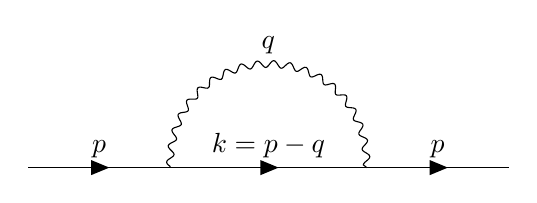
\begin{tikzpicture}
    \begin{feynman}
        \vertex (a);
        \vertex [right=1.8cm of a] (b);
        \vertex [right=2.5cm of b] (c);
        \vertex [right=1.8cm of c] (d);
        \diagram* {
            (a) -- [fermion, edge label={$p$}] (b),
            (b) -- [fermion, edge label={$k = p-q$}] (c),
            (c) -- [fermion, edge label={$p$}] (d),
            (b) -- [photon, half left, looseness=1.8, edge label={$q$}] (c)
        };
    \end{feynman}
    \end{tikzpicture}
    \caption{One-loop fermion self-energy. A fermion of momentum $p$ emits a virtual photon of momentum $q$ and propagates with $k = p - q$.}
    \label{fig:fermion_selfenergy}
\end{figure}

\noindent The relevant Feynman rules are
\begin{equation*}
    S_F(k) = \frac{i(\slashed{k} + m)}{k^2 - m^2 + i\epsilon}, \qquad
    D_{\mu\nu}(q) = \frac{-i g_{\mu\nu}}{q^2 + i\epsilon}, \qquad
    \text{vertex: } -ig\gamma^\mu,
\end{equation*}
where we use the Feynman gauge for the photon propagator and $g$ denotes the gauge coupling of the fermion. Applying these to the diagram of Figure~\ref{fig:fermion_selfenergy}, the amputated amplitude is
\begin{equation*}
    -i\Sigma(p) = \int \frac{d^d k}{(2\pi)^d}\,
    (-ig\gamma^\mu)\,\frac{i(\slashed{k} + m)}{k^2 - m^2 + i\epsilon}\,(-ig\gamma^\nu)\,
    \frac{-i g_{\mu\nu}}{(p-k)^2 + i\epsilon}.
\end{equation*}
Collecting factors of $i$ and contracting the metric,
\begin{equation}
    -i\Sigma(p) = -g^2 \int \frac{d^d k}{(2\pi)^d}\,
    \frac{\gamma^\mu(\slashed{k} + m)\gamma_\mu}{[k^2 - m^2 + i\epsilon]\,[(p-k)^2 + i\epsilon]}.
    \label{eq:Sigma_raw}
\end{equation}

\paragraph{Dirac algebra.} The numerator simplifies using the $d$-dimensional identities
\begin{equation*}
    \gamma^\mu \gamma^\nu \gamma_\mu = (2 - d)\,\gamma^\nu, \qquad
    \gamma^\mu \gamma_\mu = d.
\end{equation*}
Applying these,
\begin{equation*}
    \gamma^\mu(\slashed{k} + m)\gamma_\mu
    = (2 - d)\,\slashed{k} + d\,m.
    \label{eq:dirac_numerator}
\end{equation*}
Substituting into~\eqref{eq:Sigma_raw},
\begin{equation*}
    -i\Sigma(p) = -g^2 \int \frac{d^d k}{(2\pi)^d}\,
    \frac{(2 - d)\,\slashed{k} + d\,m}{[k^2 - m^2 + i\epsilon]\,[(p-k)^2 + i\epsilon]}.
\end{equation*}
It is convenient to split this into two pieces according to the numerator structure,
\begin{equation*}
    -i\Sigma(p) = -g^2\left[\,(2-d)\,I_k\;+\;d\,m\,I_1\,\right],
\end{equation*}
with
\begin{equation*}
    I_k \equiv \int \frac{d^d k}{(2\pi)^d}\,
    \frac{\slashed{k}}{D_1 D_2}, \qquad
    I_1 \equiv \int \frac{d^d k}{(2\pi)^d}\,
    \frac{1}{D_1 D_2},
\end{equation*}
and denominators $D_1 = k^2 - m^2 + i\epsilon$, $D_2 = (p-k)^2 + i\epsilon$.

\paragraph{Feynman parametrization.} We combine the denominators using
\begin{equation*}
    \frac{1}{D_1 D_2} = \int_0^1 dz \,\frac{1}{\big[z D_1 + (1-z) D_2\big]^2}.
\end{equation*}
Expanding the bracket,
\begin{align*}
    z D_1 + (1-z) D_2 
    &= z(k^2 - m^2) + (1-z)(p-k)^2 \nonumber\\
    &= k^2 - 2(1-z)\,p\cdot k + (1-z)p^2 - z m^2.
\end{align*}
Shifting the loop momentum, $\ell = k - (1-z)p$, completes the square:
\begin{equation*}
    z D_1 + (1-z) D_2 = \ell^2 - \Delta, \qquad
    \Delta \equiv z m^2 - z(1-z)\,p^2.
\end{equation*}

\paragraph{The vector integral $I_k$ vanishes.} Under the shift $k = \ell + (1-z)p$, the numerator of $I_k$ becomes $\slashed{\ell} + (1-z)\slashed{p}$. The piece linear in $\ell^\mu$ integrates to zero by symmetric integration in $\ell$,
\begin{equation*}
    \int \frac{d^d \ell}{(2\pi)^d}\,\frac{\ell^\mu}{[\ell^2 - \Delta]^2} = 0,
\end{equation*}
so only the $(1-z)\slashed{p}$ piece survives. Hence
\begin{equation*}
    I_k = \slashed{p}\,\int_0^1 dz\,(1-z)\,
    \int \frac{d^d \ell}{(2\pi)^d}\,\frac{1}{[\ell^2 - \Delta]^2}.
\end{equation*}

\paragraph{Performing the loop integral.} The standard result in dimensional regularization is
\begin{equation*}
    \int \frac{d^d \ell}{(2\pi)^d}\,\frac{1}{[\ell^2 - \Delta]^2}
    = \frac{i}{(4\pi)^{d/2}}\,\Gamma\!\left(2 - \tfrac{d}{2}\right)\,\Delta^{d/2 - 2}.
\end{equation*}
Setting $d = 4 - \varepsilon$ and expanding,
\begin{equation*}
    \int \frac{d^d \ell}{(2\pi)^d}\,\frac{1}{[\ell^2 - \Delta]^2}
    = \frac{i}{(4\pi)^2}\left[\frac{2}{\varepsilon} - \gamma_E + \ln(4\pi) - \ln\!\frac{\Delta}{\mu^2} + \mathcal{O}(\varepsilon)\right],
\end{equation*}
where $\mu$ has been introduced via $g \to g\,\mu^{\varepsilon/2}$ to preserve the mass dimension of the coupling.

\paragraph{Assembling $\Sigma(p)$.} Collecting the two pieces and using $(2-d) = -2 + \varepsilon$, $d = 4 - \varepsilon$,
\begin{equation}
    \Sigma(p) = \frac{g^2}{(4\pi)^2}\int_0^1 dz\,
    \Big[\,(\varepsilon - 2)(1-z)\,\slashed{p} \;+\; (4 - \varepsilon)\,m\,\Big]\,
    \left[\frac{2}{\varepsilon} - \gamma_E + \ln(4\pi) - \ln\!\frac{\Delta}{\mu^2}\right].
    \label{eq:Sigma_assembled}
\end{equation}

\subsection*{Mass renormalization and the protection structure}

The bare mass $m_0$ and the renormalized mass $m$ are related by $m_0 = m + \delta m$, with $\delta m$ chosen to enforce the on-shell condition: the full propagator has a pole at $\slashed{p} = m$, i.e.\
\begin{equation*}
    \Sigma_R(\slashed{p} = m) = 0, \qquad
    \Sigma_R(p) \equiv \Sigma(p) - \delta m.
\end{equation*}
Imposing this on~\eqref{eq:Sigma_assembled} gives
\begin{equation*}
    \delta m = \Sigma(\slashed{p} = m)
    = \frac{g^2\,m}{(4\pi)^2}\int_0^1 dz\,
    \Big[\,(4-\varepsilon) - (2-\varepsilon)(1-z)\,\Big]\,
    \left[\frac{2}{\varepsilon} + \text{finite}\right],
\end{equation*}
which evaluates to a divergent piece plus finite logarithms:
\begin{equation*}
    \;\delta m \;=\; \frac{3g^2\,m}{(4\pi)^2}\,
    \left[\frac{2}{\varepsilon} + \text{finite} - \ln\!\frac{m^2}{\mu^2}\right]\;,
\end{equation*}
where we highlight the proportionality:
\begin{equation*}
    \boxed{\;\delta m \propto m.\ }
\end{equation*}

\subsection{Scalar Self-energy}
\label{app:scalar_selfenergy}

Now, to find the scalar mass correction, consider the one-loop scalar self-energy in Yukawa theory. In particular, a fermion and an antifermion loop between the two Yukawa vertices, with two scalar external legs of momentum $p$. Diagrammatically,

\begin{figure}[H]
    \centering
    \begin{tikzpicture}
    \begin{feynman}
        \vertex (a);
        \vertex [right=1.8cm of a] (b);
        \vertex [right=2cm of b] (c);
        \vertex [right=1.8cm of c] (d);
        \diagram* {
            (a) -- [scalar, edge label={$p$}] (b),
            (b) -- [fermion, half left, looseness=1.6, edge label={$k$}] (c),
            (c) -- [fermion, half left, looseness=1.6, edge label={$k+p$}] (b),
            (c) -- [scalar, edge label={$p$}] (d)
        };
    \end{feynman}
    \end{tikzpicture}
    \caption{One-loop scalar self-energy from a fermion loop in Yukawa theory. A fermion of momentum $k$ and a fermion of momentum $k+p$ circulate in the loop between the two Yukawa vertices.}
    \label{fig:scalar_selfenergy}
\end{figure}

\noindent The relevant Feynman rules are
\begin{equation*}
    S_F(k) = \frac{i(\slashed{k}+m_\psi)}{k^2-m_\psi^2+i\epsilon}, \qquad
    \text{vertex: } -iy,
\end{equation*}
coming from the Yukawa interaction $\mathcal{L}\supset -y\,\phi\,\bar\psi\psi$. Applying these to the diagram of Figure~\ref{fig:scalar_selfenergy} and including the mandatory factor of $(-1)$ for the closed fermion loop together with a trace over Dirac indices, the amputated amplitude is
\begin{equation*}
    -i\Sigma_\phi(p^2) = -(-iy)^2\,\mathrm{Tr}\int\frac{d^dk}{(2\pi)^d}\,
    \frac{i(\slashed{k}+m_\psi)}{k^2-m_\psi^2+i\epsilon}\,
    \frac{i(\slashed{k}+\slashed{p}+m_\psi)}{(k+p)^2-m_\psi^2+i\epsilon}.
\end{equation*}
Collecting factors of $i$,
\begin{equation}
    i\Sigma_\phi(p^2) = y^2\int\frac{d^dk}{(2\pi)^d}\,
    \frac{\mathrm{Tr}\big[(\slashed{k}+m_\psi)(\slashed{k}+\slashed{p}+m_\psi)\big]}
    {[k^2-m_\psi^2+i\epsilon]\,[(k+p)^2-m_\psi^2+i\epsilon]}.
    \label{eq:SigmaPhi_raw}
\end{equation}

\paragraph{Trace algebra.} Using $\mathrm{Tr}[\gamma^\mu\gamma^\nu]=4g^{\mu\nu}$, $\mathrm{Tr}[\textbf{1}]=4$ and that an odd number of gamma matrices traces to zero,
\begin{equation}
    \mathrm{Tr}\big[(\slashed{k}+m_\psi)(\slashed{k}+\slashed{p}+m_\psi)\big]
    = 4\big[k\cdot(k+p) + m_\psi^2\big].
    \label{eq:trace_numerator}
\end{equation}
Substituting into~\eqref{eq:SigmaPhi_raw},
\begin{equation*}
    i\Sigma_\phi(p^2) = 4y^2\int\frac{d^dk}{(2\pi)^d}\,
    \frac{k\cdot(k+p)+m_\psi^2}{D_1 D_2},
\end{equation*}
with $D_1 = k^2-m_\psi^2+i\epsilon$, $D_2 = (k+p)^2-m_\psi^2+i\epsilon$. Unlike the fermion self-energy, there is no leftover Dirac structure here: the trace has already reduced the numerator to a pure scalar function of $k$ and $p$.

\paragraph{Feynman parametrization.} Combining denominators as before,
\begin{equation*}
    \frac{1}{D_1 D_2} = \int_0^1 dz\,\frac{1}{\big[z D_1+(1-z) D_2\big]^2},
\end{equation*}
and shifting $\ell = k+(1-z)p$ completes the square:
\begin{equation*}
    z D_1+(1-z) D_2 = \ell^2-\Delta, \qquad
    \Delta \equiv m_\psi^2 - z(1-z)\,p^2.
\end{equation*}
Under the same shift, $k\cdot(k+p) \to \ell^2 + (2z-1)\,\ell\cdot p - z(1-z)p^2$. The term linear in $\ell^\mu$ vanishes by symmetric integration and using $m_\psi^2-z(1-z)p^2=\Delta$ the numerator collapses to
\begin{equation*}
    k\cdot(k+p)+m_\psi^2 \;\longrightarrow\; \ell^2+\Delta.
\end{equation*}
Hence, writing $\ell^2+\Delta = (\ell^2-\Delta)+2\Delta$,
\begin{equation*}
    i\Sigma_\phi(p^2) = 4y^2\int_0^1 dz\left[\int\frac{d^d\ell}{(2\pi)^d}\frac{1}{\ell^2-\Delta}
    + 2\Delta\int\frac{d^d\ell}{(2\pi)^d}\frac{1}{[\ell^2-\Delta]^2}\right].
\end{equation*}

\paragraph{Performing the loop integrals.} The standard dimensional-regularization master formula,
\begin{equation*}
    \int\frac{d^d\ell}{(2\pi)^d}\frac{1}{[\ell^2-\Delta]^n}
    = \frac{(-1)^n i}{(4\pi)^{d/2}}\,\frac{\Gamma(n-\tfrac d2)}{\Gamma(n)}\,\Delta^{d/2-n},
\end{equation*}
reproduces the $n=2$ result used in the fermion calculation,
\begin{equation*}
    \int\frac{d^d\ell}{(2\pi)^d}\frac{1}{[\ell^2-\Delta]^2}
    = \frac{i}{(4\pi)^2}\left[\frac{2}{\varepsilon}-\gamma_E+\ln(4\pi)-\ln\frac{\Delta}{\mu^2}+\mathcal{O}(\varepsilon)\right],
\end{equation*}
while the $n=1$ piece, using the recursion $\Gamma(z-1)=\Gamma(z)/(z-1)$ on $\Gamma(1-\tfrac d2)=\Gamma(-1+\tfrac\varepsilon2)$, picks up an extra finite shift relative to the $n=2$ case:
\begin{equation*}
    \int\frac{d^d\ell}{(2\pi)^d}\frac{1}{\ell^2-\Delta}
    = \frac{i\,\Delta}{(4\pi)^2}\left[\frac{2}{\varepsilon}+1-\gamma_E+\ln(4\pi)-\ln\frac{\Delta}{\mu^2}+\mathcal{O}(\varepsilon)\right].
\end{equation*}
The crucial difference from the fermion calculation is that this integral carries an overall power of $\Delta$ outside the bracket.

\paragraph{Assembling $\Sigma_\phi(p^2)$.} Combining both pieces,
\begin{equation}
    \Sigma_\phi(p^2) = \frac{4y^2}{(4\pi)^2}\int_0^1 dz\,\Delta(z,p^2)\,
    \left\{1+3\left[\frac{2}{\varepsilon}-\gamma_E+\ln(4\pi)-\ln\frac{\Delta(z,p^2)}{\mu^2}\right]\right\},
    \label{eq:SigmaPhi_assembled}
\end{equation}
with $\Delta(z,p^2)=m_\psi^2-z(1-z)p^2$.

\subsection*{Mass renormalization and the lack of protection structure}

The bare mass $m_{\phi,0}^2$ and renormalized mass $m_\phi^2$ are related by $m_{\phi,0}^2 = m_\phi^2+\delta m_\phi^2$, with $\delta m_\phi^2$ fixed by the renormalization condition $\widetilde\Gamma_R^{(2)}(p^2{=}0)=m_\phi^2$, i.e.
\begin{equation*}
    \Sigma_{\phi,R}(0) = \Sigma_\phi(0)-\delta m_\phi^2 = 0
    \qquad\Longrightarrow\qquad
    \delta m_\phi^2 = \Sigma_\phi(0).
\end{equation*}
At $p^2=0$, $\Delta(z,0)=m_\psi^2$ for every $z$, so the parameter integral in~\eqref{eq:SigmaPhi_assembled} trivializes and
\begin{align*}
    \delta m_\phi^2 &= \frac{4y^2 m_\psi^2}{(4\pi)^2}
    \left\{1+3\left[\frac{2}{\varepsilon}-\gamma_E+\ln(4\pi)-\ln\frac{m_\psi^2}{\mu^2}\right]\right\}\\
    &=\;
    \frac{12\,y^2 m_\psi^2}{(4\pi)^2}\left[\frac{2}{\varepsilon}+\frac13-\gamma_E+\ln(4\pi)-\ln\frac{m_\psi^2}{\mu^2}\right].
\end{align*}
Unlike the fermion case, where $\delta m$ was proportional to $m$ itself, here the external scalar mass $m_\phi$ never entered the loop at all, the only mass running through the diagram is the fermion mass $m_\psi$. The divergence attaches itself entirely to $m_\psi^2$, then:
\begin{equation*}
    \boxed{\;\delta m_\phi^2 \;\slashed{\propto}\; m_\phi^2.\;}
\end{equation*}

\acknowledgments
I would like to thank my advisor, Jordi Salvadó Serra, for his guidance, and for always making room for one more question. His insight and enthusiasm shaped this work.

\noindent Finally, to my family and friends: thank you for being my orbit of stability during this degree.

\begin{thebibliography}{99}

\bibitem{PeskinHierarchy} Peskin, M.~E. "What is the Hierarchy Problem?" Nuclear Physics B {\bf 1018}: 116971 (2025).

\bibitem{2HDM} Ferreira, P.~M., Grzadkowski, B., Ogreid, O.~M., and Osland, P. "New symmetries of the two-Higgs-doublet model." The European Physical Journal C {\bf 84}: 234 (2024).

\bibitem{Trautner_goofy1} Trautner, A. "Goofy transformations and the hierarchy problem." Physics Letters B {\bf 873}: 140190 (2026).

\bibitem{goofy2} de Boer, T., Goertz, F., and Incrocci, A. "The goofy-symmetric Standard Model and the hierarchy problem." arXiv:2507.22111 [hep-ph] (2025).

\bibitem{CraigNaturalness} Craig, N. "Naturalness: Past, Present and Future." The European Physical Journal C {\bf 83}: 825 (2023).

\bibitem{wilson} Wilson, K.~G. "The Renormalization Group and Strong Interactions." Physical Review D {\bf 3}: 1818--1846 (1971).

\bibitem{FerreiraHPNP2023} Ferreira, P.~M. "GOOFy Symmetries of the Two Higgs Doublet Model." Presentation at the 6th International Workshop on Higgs as a Probe of New Physics (HPNP2023), Osaka University, Osaka, Japan, 5 June 2023.

\bibitem{deBoer_Trautner_Outs} de Boer, T. and Trautner, A. "Outer automorphisms are sufficient conditions for RG fixed points." arXiv:2603.12318 [hep-th] (2026).

\bibitem{blocking} Di Carlo, L. "Monte Carlo, blocking, and inference: How to measure the renormalization group flow." American Journal of Physics {\bf 92}: 447 (2024).

\bibitem{TrautnerGoofy} Trautner, A. "Goofy transformations \& RG fixed points." Planck'26 Conference, CERN (2026).

\bibitem{bilinear_2HDM} Ivanov, I.~P. "Minkowski space structure of the Higgs potential in 2HDM." Physical Review D {\bf 75}: 035001 (2007). [Erratum: Physical Review D {\bf 76}: 039902 (2007).]

\bibitem{Goldenfeld} Goldenfeld, N. \textsl{Lectures on Phase Transitions and the Renormalization Group}, Frontiers in Physics Vol.~85 (Addison-Wesley, Reading, MA, 1992).

\bibitem{Cardy} Cardy, J. \textsl{Scaling and Renormalization in Statistical Physics}, Cambridge Lecture Notes in Physics Vol.~5 (Cambridge University Press, Cambridge, 1996).

\bibitem{TongSFT} Tong, D. "Statistical Field Theory." Lecture Notes, University of Cambridge (2023).

\bibitem{KorenHierarchy} Koren, S. \textsl{The Hierarchy Problem: From the Fundamentals to the Frontiers}, PhD thesis, University of California, Santa Barbara (2020).

\end{thebibliography}

\end{document}